\documentclass[11pt,a4paper]{article}
\usepackage[margin={2.6cm,2.6cm}]{geometry}
\usepackage{lmodern}
\usepackage{microtype}
\usepackage{enumitem}
\usepackage{array}
\usepackage[spanish,es-tabla]{babel}
\usepackage[utf8]{inputenc}
\usepackage[T1]{fontenc}
\usepackage{amsmath, amsthm, amsfonts}
\usepackage{hyperref}
\usepackage{xcolor}
\usepackage{graphicx}
 \usepackage{float}
\usepackage{listings}
\usepackage{fontawesome5}
\usepackage{dirtree}

\spanishdecimal{.}


\definecolor{azuluc}{HTML}{1F4E79}
\definecolor{grisclaro}{HTML}{F4F6F8}
\definecolor{gris}{HTML}{586069}
\definecolor{verde}{HTML}{2E7D32}
\definecolor{rojo}{HTML}{A94442}
\definecolor{git}{HTML}{F1502F}

\definecolor{morado_ubuntu}{RGB}{48, 10, 36}       % Fondo morado oscuro de Ubuntu GNOME
\definecolor{verde_ubuntu}{RGB}{78, 154, 6}        % Verde para comentarios
\definecolor{cyan_ubuntu}{RGB}{52, 226, 226}       % Cian para comandos
\definecolor{amarillo_ubuntu}{RGB}{250, 240, 190}  % Amarillo para cadenas
\definecolor{rojo_ubuntu}{RGB}{220, 50, 47}        % Rojo para errores
\definecolor{verde_claro_ubuntu}{RGB}{138, 226, 52} % Verde claro para el prompt
\definecolor{azul_ubuntu}{RGB}{114, 159, 207}      % Azul para símbolos y rutas
\definecolor{gris_ubuntu}{RGB}{128, 128, 128}      % Gris para el borde del frame


\definecolor{fondo_mac}{RGB}{255, 255, 250}       % Fondo beige claro típico de macOS
\definecolor{negro}{RGB}{0, 0, 0}                 % Texto en negro
\definecolor{verde_mac}{RGB}{63, 127, 95}         % Verde para comentarios
\definecolor{azul_mac}{RGB}{0, 0, 255}            % Azul para comandos y prompt
\definecolor{rojo_mac}{RGB}{196, 26, 22}          % Rojo para errores y cadenas
\definecolor{morado_mac}{RGB}{147, 39, 143}       % Morado para emphasis (opcional)
\definecolor{gris_mac}{RGB}{200, 200, 200}        % Gris para el borde del frame

\definecolor{DarkGreen}{RGB}{0,102,0}
\definecolor{DarkYellow}{RGB}{243,220,12}



\lstdefinestyle{rstyle}{
  language=R,
  basicstyle=\ttfamily\small,
  keywordstyle=\color{azuluc}\bfseries,
  commentstyle=\color{gris},
  stringstyle=\color{verde!70!black},
  showstringspaces=false,
  frame=single,
  rulecolor=\color{gris!30},
  backgroundcolor=\color{grisclaro},
  breaklines=true,
  showspaces=false,
  tabsize=2,
    literate=
    {á}{{\'a}}1
    {é}{{\'e}}1
    {í}{{\'i}}1
    {ó}{{\'o}}1
    {ú}{{\'u}}1
    {Á}{{\'A}}1
    {É}{{\'E}}1
    {Í}{{\'I}}1
    {Ó}{{\'O}}1
    {Ú}{{\'U}}1
    {ñ}{{\~n}}1
    {Ñ}{{\~N}}1
    {ü}{{\"u}}1
    {Ü}{{\"U}}1
    {¡}{{\textexclamdown}}1
	{`}{\textasciigrave}1 
    {´}{\textquotesingle}1,
}

\lstdefinestyle{rconsole}{
  language=R,
  basicstyle=\color{rojo}\ttfamily\small,
  showstringspaces=false,
  frame=single,
  rulecolor=\color{gris!30},
  breaklines=true,
  tabsize=2,
  literate=
    {á}{{\'a}}1
    {é}{{\'e}}1
    {í}{{\'i}}1
    {ó}{{\'o}}1
    {ú}{{\'u}}1
    {Á}{{\'A}}1
    {É}{{\'E}}1
    {Í}{{\'I}}1
    {Ó}{{\'O}}1
    {Ú}{{\'U}}1
    {ñ}{{\~n}}1
    {Ñ}{{\~N}}1
    {ü}{{\"u}}1
    {Ü}{{\"U}}1
    {¡}{{\textexclamdown}}1
	{`}{\textasciigrave}1 
    {´}{\textquotesingle}1,
}

\lstdefinestyle{routput}{
  language=R,
  basicstyle=\color{azuluc}\ttfamily\small,
  showstringspaces=false,
  frame=single,
  rulecolor=\color{gris!30},
  breaklines=true,
  tabsize=2,
  literate=
    {á}{{\'a}}1
    {é}{{\'e}}1
    {í}{{\'i}}1
    {ó}{{\'o}}1
    {ú}{{\'u}}1
    {Á}{{\'A}}1
    {É}{{\'E}}1
    {Í}{{\'I}}1
    {Ó}{{\'O}}1
    {Ú}{{\'U}}1
    {ñ}{{\~n}}1
    {Ñ}{{\~N}}1
    {ü}{{\"u}}1
    {Ü}{{\"U}}1
    {¡}{{\textexclamdown}}1
	{`}{\textasciigrave}1 
    {´}{\textquotesingle}1,
}

\lstdefinestyle{mdstyle}{
  basicstyle=\ttfamily\footnotesize,
  keywordstyle=\color{azuluc}\bfseries,
  commentstyle=\color{gris},
  showstringspaces=false,
  showspaces=false,
  tabsize=2,
  frame=single,
  rulecolor=\color{gris!30},
  backgroundcolor=\color{grisclaro},
  breaklines=true,
  breakatwhitespace=false,
  % Títulos Markdown
  morecomment=[l][\color{azuluc}\bfseries]{\#},
  % Enlaces y referencias
  morecomment=[s][\color{verde}]{(}{)},
  % Cadenas
  morestring=[b][\color{naranja}]{"},
  morestring=[b][\color{naranja}]{'},
  % Lenguajes utilizados en bloques de código
  classoffset=1,
    keywordstyle=\color{morado}\bfseries,
    morekeywords={python,bash,R,latex,json,yaml},
  classoffset=0,
  % Protocolos y enlaces
  emph={http,https,ftp},
  escapeinside={-@}{@-},
  emphstyle=\color{azuluc}\underbar,   
   literate=
    {á}{{\'a}}1
    {é}{{\'e}}1
    {í}{{\'i}}1
    {ó}{{\'o}}1
    {ú}{{\'u}}1
    {Á}{{\'A}}1
    {É}{{\'E}}1
    {Í}{{\'I}}1
    {Ó}{{\'O}}1
    {Ú}{{\'U}}1
    {ñ}{{\~n}}1
    {Ñ}{{\~N}}1
    {ü}{{\"u}}1
    {Ü}{{\"U}}1
    {¡}{{\textexclamdown}}1
	{`}{\textasciigrave}1 
    {´}{\textquotesingle}1,
}

\lstdefinestyle{ubuntugnome}{
  basicstyle=\ttfamily\small\color{white},
  backgroundcolor=\color{morado_ubuntu},
  commentstyle=\color{verde_ubuntu},
  keywordstyle=\color{cyan_ubuntu},
  stringstyle=\color{amarillo_ubuntu},
  emphstyle=\color{rojo_ubuntu},
  showstringspaces=false,
  frame=single,
  rulecolor=\color{gris_ubuntu},
  breaklines=true,
  postbreak=\mbox{\textcolor{white}{$\hookrightarrow$}\space},
  % Configuración para simular el prompt de Ubuntu
  upquote=true,
  % Resaltar el prompt de usuario
  emph={user@ubuntu:~\$},
  emphstyle={\color{verde_claro_ubuntu}\bfseries},
  % Resaltar errores (ej: "command not found")
  classoffset=1,
  emph={command not found,No such file or directory,Permission denied},
  emphstyle={\color{rojo_ubuntu}},
  classoffset=0,
}

\lstdefinestyle{macterminal}{
  basicstyle=\ttfamily\small\color{negro},
  backgroundcolor=\color{fondo_mac},
  commentstyle=\color{verde_mac},
  keywordstyle=\color{azul_mac},
  stringstyle=\color{rojo_mac},
  emphstyle=\color{morado_mac},
  showstringspaces=false,
  frame=single,
  rulecolor=\color{gris_mac},
  breaklines=true,
  postbreak=\mbox{\textcolor{negro}{$\hookrightarrow$}\space},
  % Configuración para simular el prompt de macOS
  upquote=true,
  % Resaltar el prompt de usuario
  emphstyle={\color{azul_mac}\bfseries},
  % Resaltar errores (ej: "command not found")
  classoffset=1,
  emph={command not found,No such file or directory,Permission denied},
  emphstyle={\color{rojo_mac}},
  classoffset=0
}

\lstdefinestyle{windowscmd}{
  basicstyle=\ttfamily\small\color{white},
  backgroundcolor=\color{black},
  showstringspaces=false,
  frame=single,
  rulecolor=\color{gris_mac},
  breaklines=true,
  postbreak=\mbox{\textcolor{negro}{$\hookrightarrow$}\space},
  % Configuración para simular el prompt de macOS
  upquote=true,
  % Resaltar el prompt de usuario
  emphstyle={\color{azul_mac}\bfseries},
  % Resaltar errores (ej: "command not found")
  classoffset=1,
  emph={command not found,No such file or directory,Permission denied},
  emphstyle={\color{rojo_mac}},
  classoffset=0
}



\newcommand*{\vsp}{\texttt{\textvisiblespace}} % visible space

\newcommand*{\strC}{\begingroup
  \obeyspaces
  \begingroup\lccode`~=`\ %
  \lowercase{\endgroup\let~}\vsp
  \dostrC}
\newcommand{\dostrC}[1]{\textnormal{{\slshape\ttfamily#1}}\endgroup} % string constant


\newcommand{\R}{\textcolor{azuluc}{\faIcon{r-project}}}
\newcommand{\Git}{\textcolor{git}{\faIcon{git-alt}}~\!Git}
\newcommand{\GitHub}{\faIcon{github}~\!GitHub}
\newcommand{\Markdown}{Markdown~\faIcon{markdown}}



\newcommand{\checkicon}{\textcolor{verde}{\faIcon{check}}}
\newcommand{\crossicon}{\textcolor{rojo}{\faIcon{times}}}

\newtheoremstyle{exercise}
  {0.8em}{0.8em}{\normalfont}{}{\bfseries\color{azuluc}}{.}{0.5em}{}
\theoremstyle{exercise}
\newtheorem{exercise}{Ejercicio}

\title{\LARGE\textbf{Práctica 7: Gráficos en \R}\\[0.5em]
\Large Laboratorio de Matemáticas\\
\small\ \\
\Large Grado en Ingeniería Matemática - Doble Grado en Física e Ingeniería Matemática}
\author{Miguel Beltra Vidal}
\date{Curso 2026/27}

\begin{document}
\maketitle

\section{Objetivos}

El objetivo de esta práctica es aprender a crear gráficos utilizando \R. para representar información mediante gráficos. Al acabar la práctica, el estudiante podrá representar cualquier gráfico que necesite para sus trabajos usando \R.


\section[Primeros gráficos en R]{Primeros gráficos en \R}

\subsection{Función \texttt{plot}}

\R\ permite crear gráficos directamente a partir de vectores. Una de las funciones fundamentales es \texttt{plot()}. A esta función tenemos que especificarle las coordenadas $x$ y las coordenadas $y$ de los puntos que queremos que dibuje. Por ejemplo, las siguientes instrucciones:

\begin{lstlisting}[style=rstyle]
x <- seq(-10, 10, by=0.25)
y <- sin(x)
plot(x,y)
\end{lstlisting}

\noindent tienen como salida:

\begin{center}
	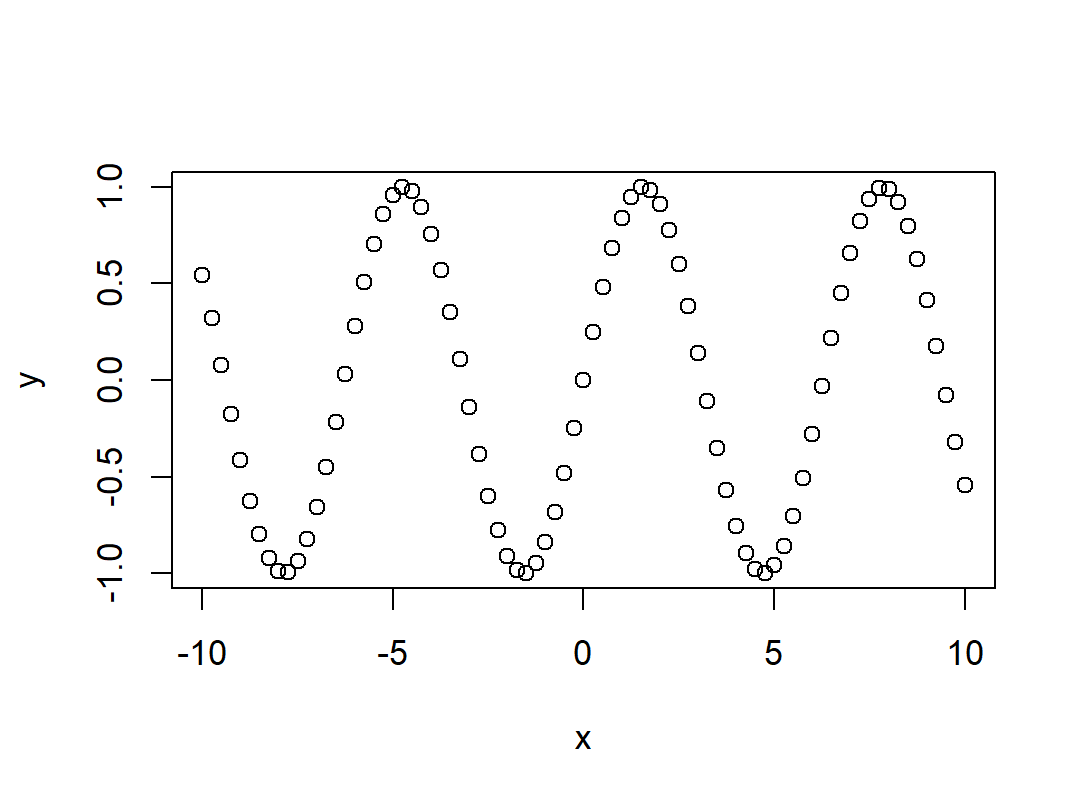
\includegraphics[width=0.75\linewidth,trim={0 0 0 1cm},clip]{images/sinus_plot_1.png}
\end{center}


En RStudio los gráficos generados se mostrarán en la esquina inferior derecha. Desde esta misma ventana podemos exportar los gráficos que generemos desde el botón \texttt{Export}.

\begin{center}
	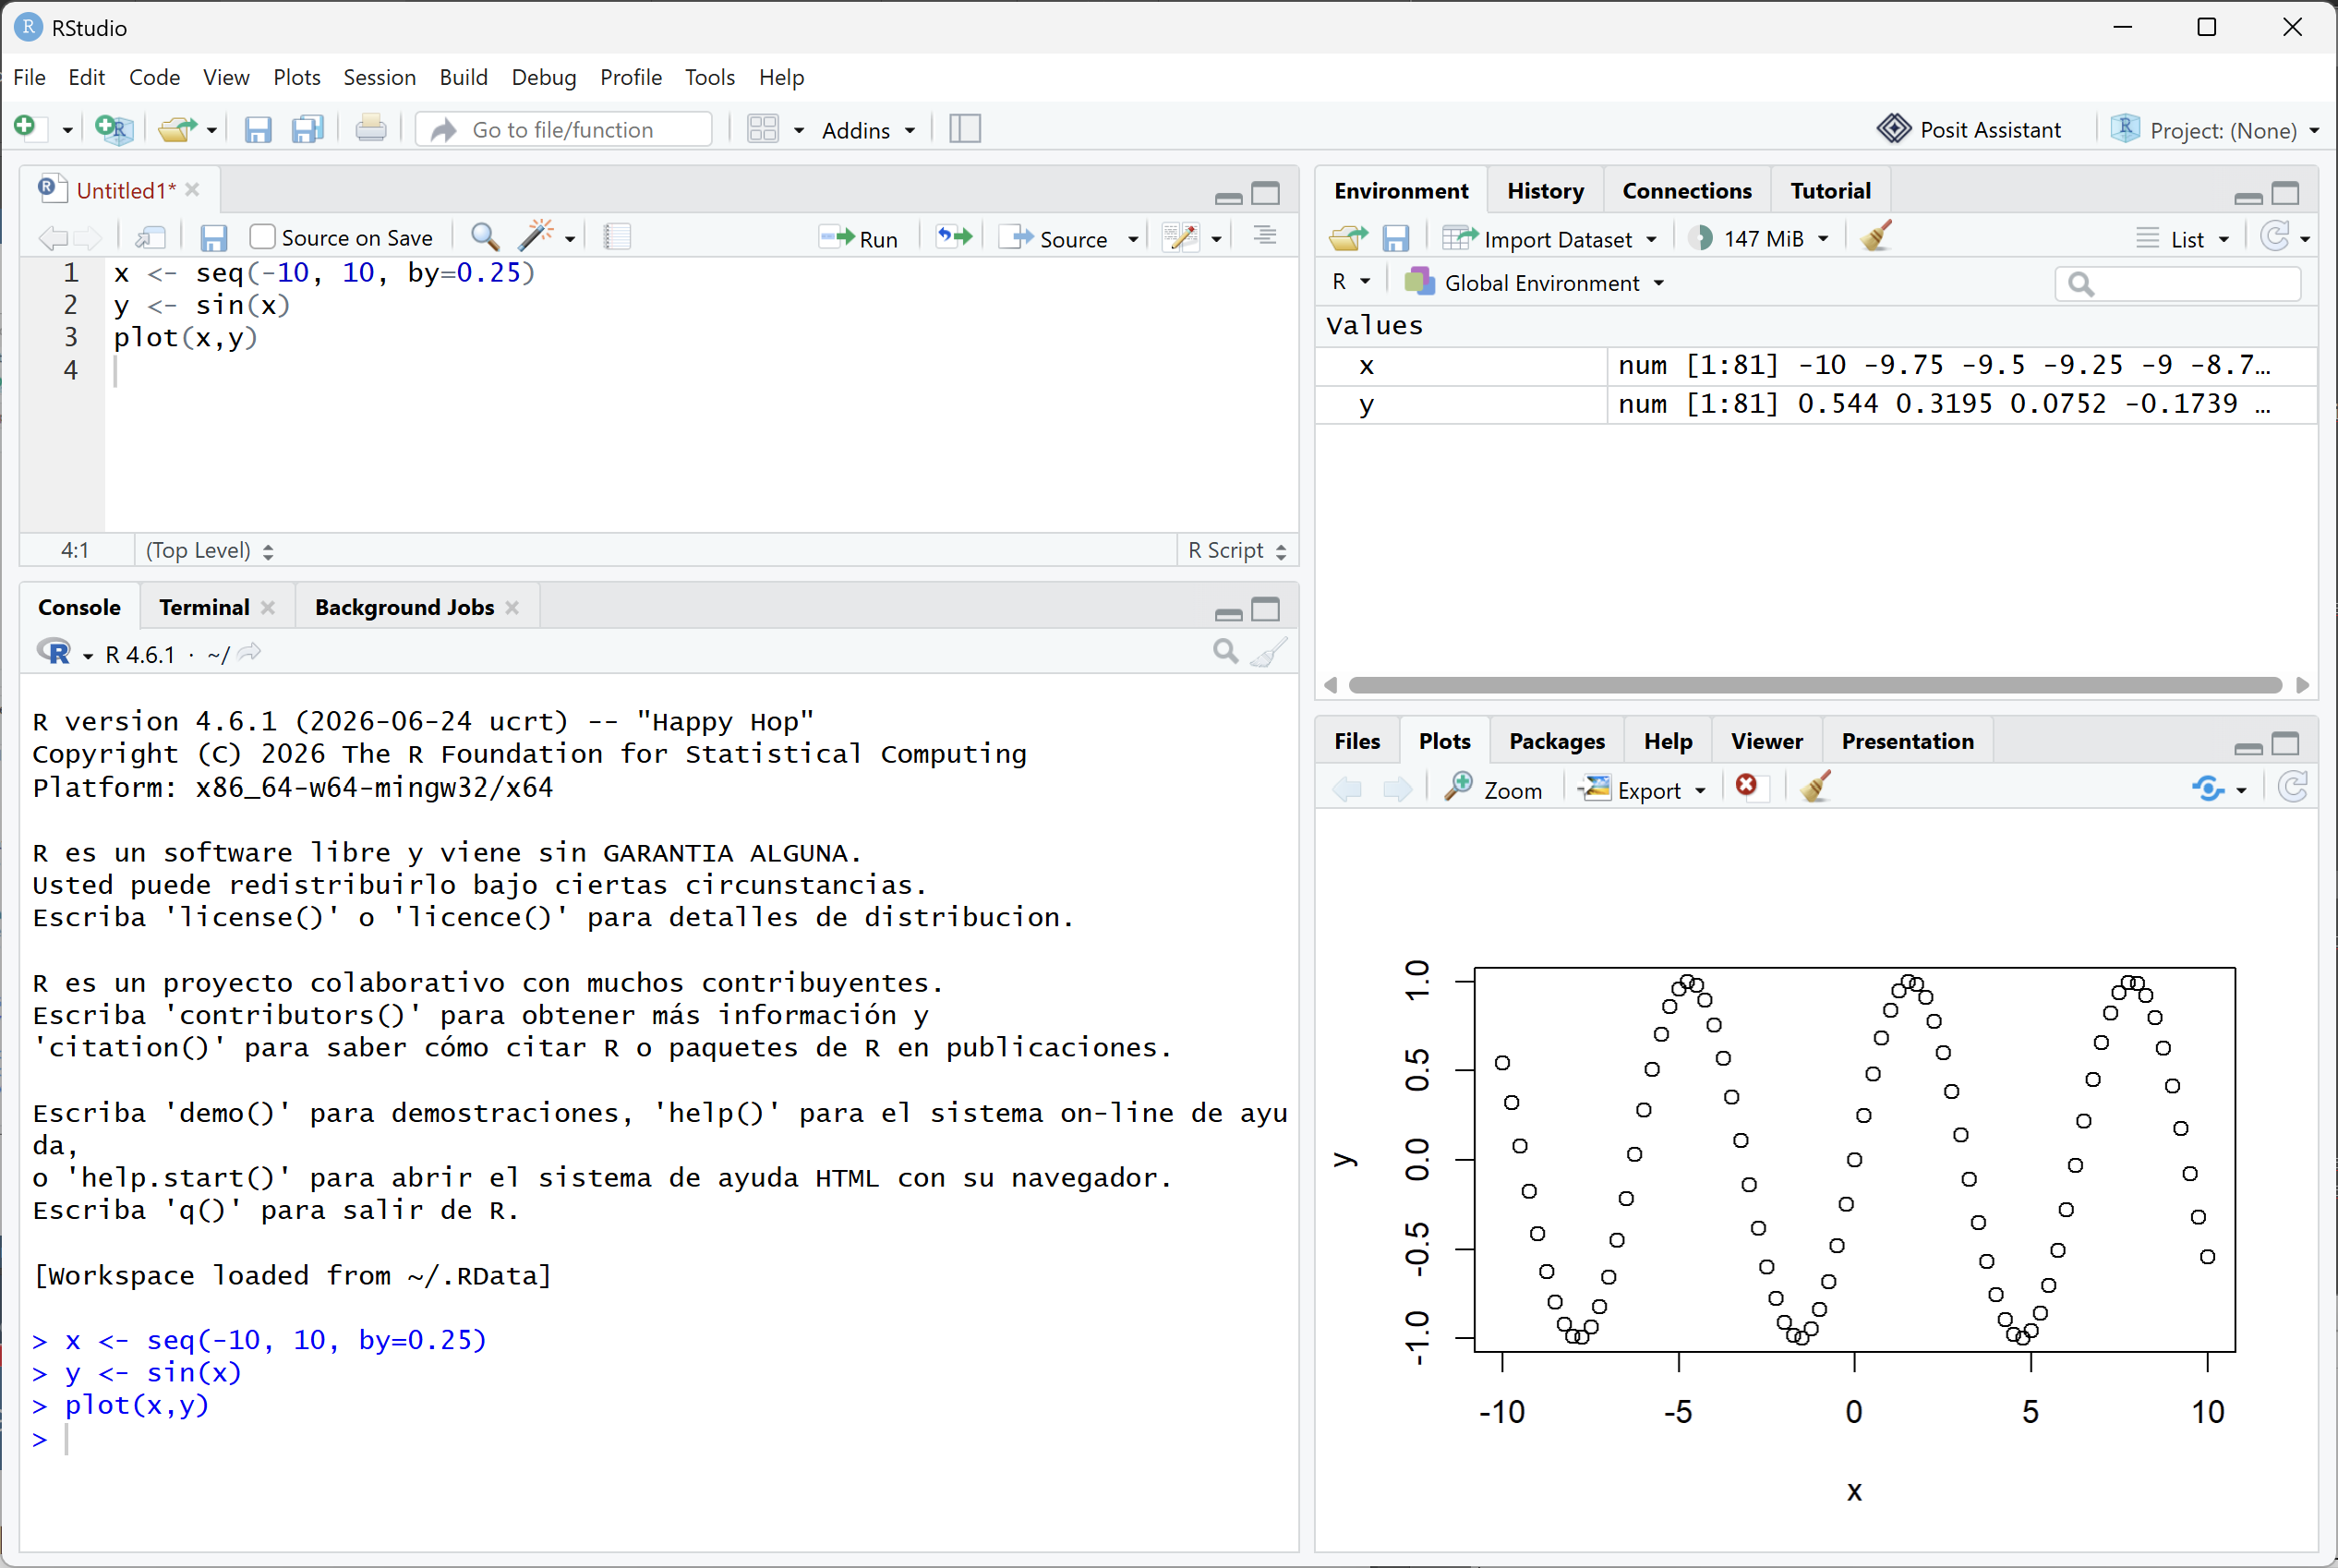
\includegraphics[width=0.75\linewidth]{images/RStudio_plot.png}
\end{center}


Podemos añadir más puntos para obtener mejores gráficas. Las siguientes gráficas se corresponden con las siguientes instrucciones:

\bigskip

\noindent
\begin{minipage}{0.45\linewidth}
\begin{lstlisting}[style=rstyle]
x <- seq(-10, 10, by=0.5)
y <- sin(x)
plot(x,y)
\end{lstlisting}
\begin{center}
	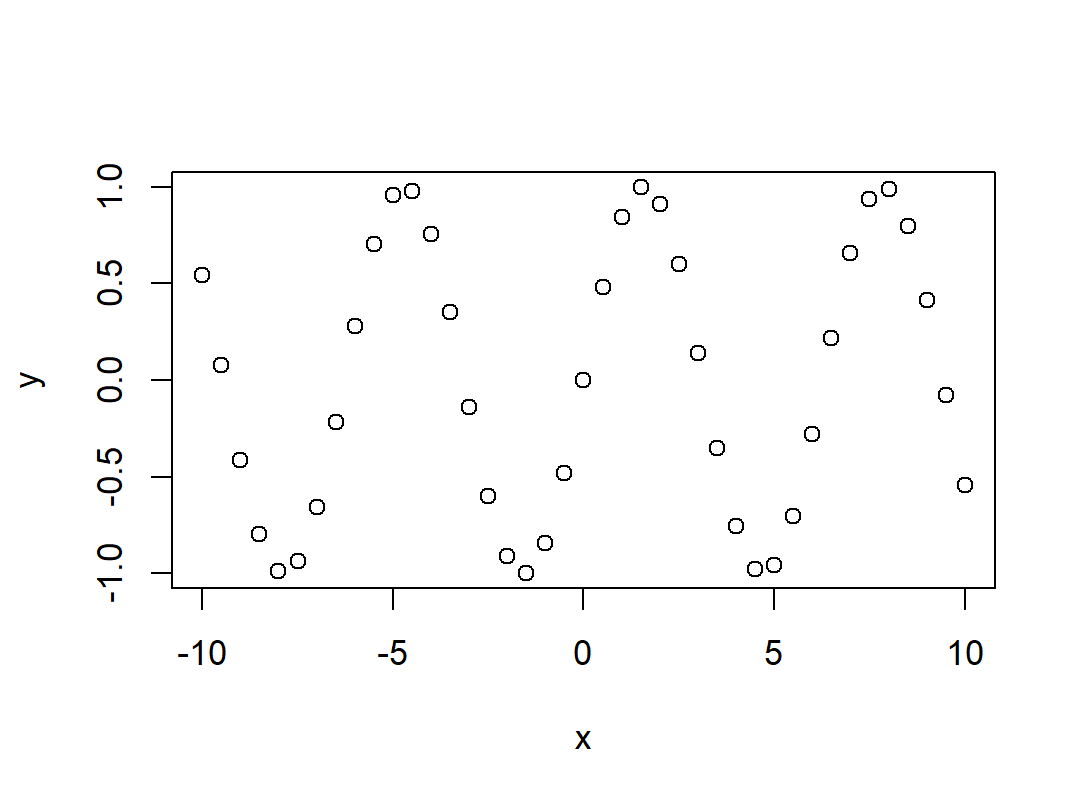
\includegraphics[width=\linewidth,trim={0 0 0 2cm},clip]{images/sinus_plot_0.png}
\end{center}
\end{minipage}
~
\hspace{0.5cm}
~
\begin{minipage}{0.45\textwidth}
\begin{lstlisting}[style=rstyle]
x <- seq(-10, 10, by=0.25)
y <- sin(x)
plot(x,y)
\end{lstlisting}

\begin{center}
	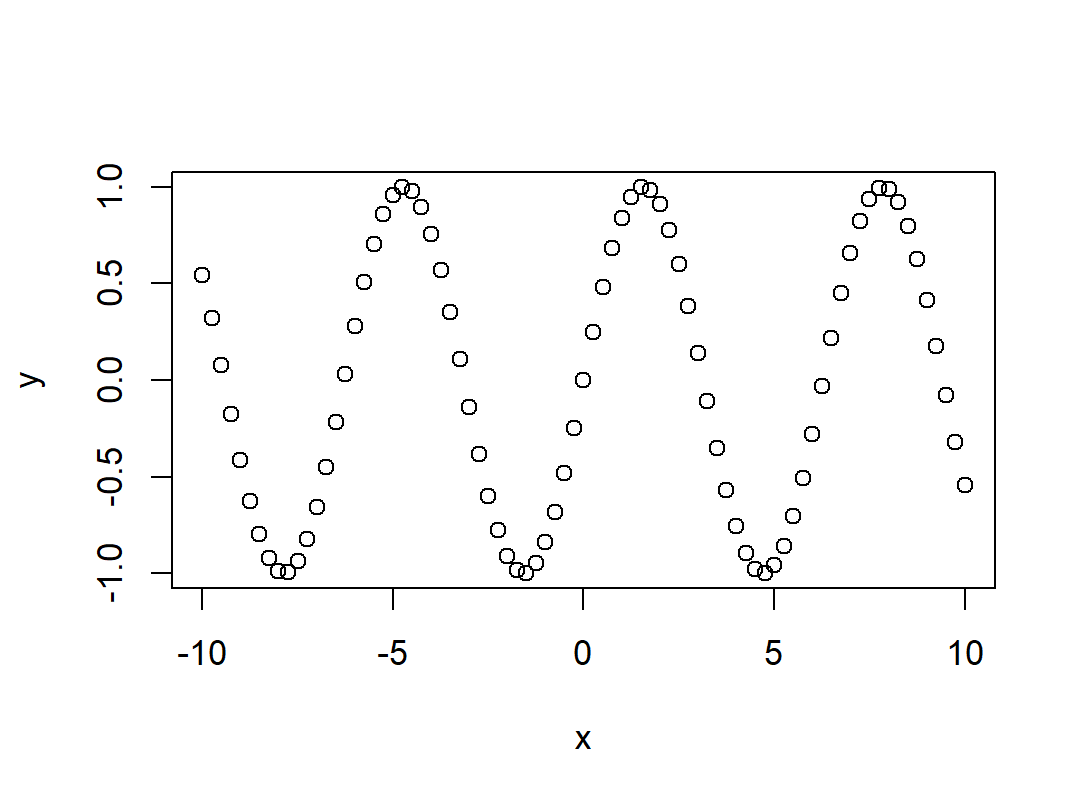
\includegraphics[width=\linewidth,trim={0 0 0 2cm},clip]{images/sinus_plot_1.png}
\end{center}
\end{minipage}

\noindent
\begin{minipage}{0.45\linewidth}
\begin{lstlisting}[style=rstyle]
x <- seq(-10, 10, by=0.1)
y <- sin(x)
plot(x,y)
\end{lstlisting}
\begin{center}
	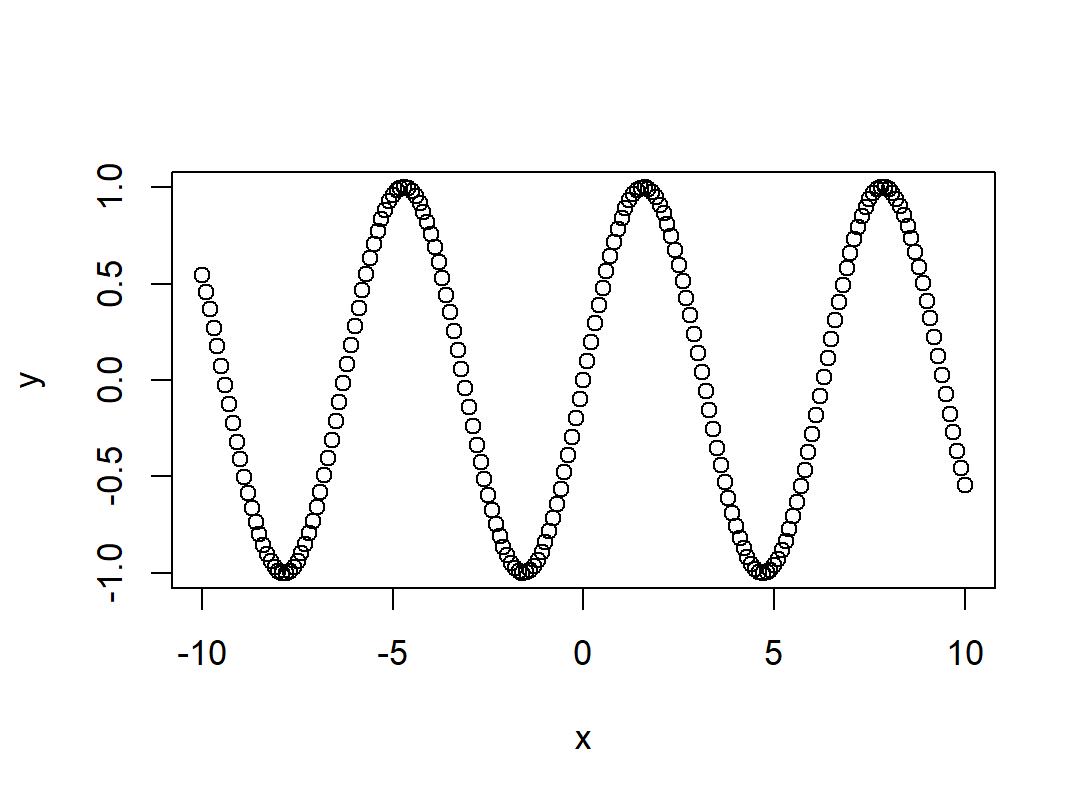
\includegraphics[width=\linewidth,trim={0 0 0 2cm},clip]{images/sinus_plot_2.png}
\end{center}
\end{minipage}
~
\hspace{0.5cm}
~
\begin{minipage}{0.45\textwidth}
\begin{lstlisting}[style=rstyle]
x <- seq(-10, 10, by=0.01)
y <- sin(x)
plot(x,y)
\end{lstlisting}

\begin{center}
	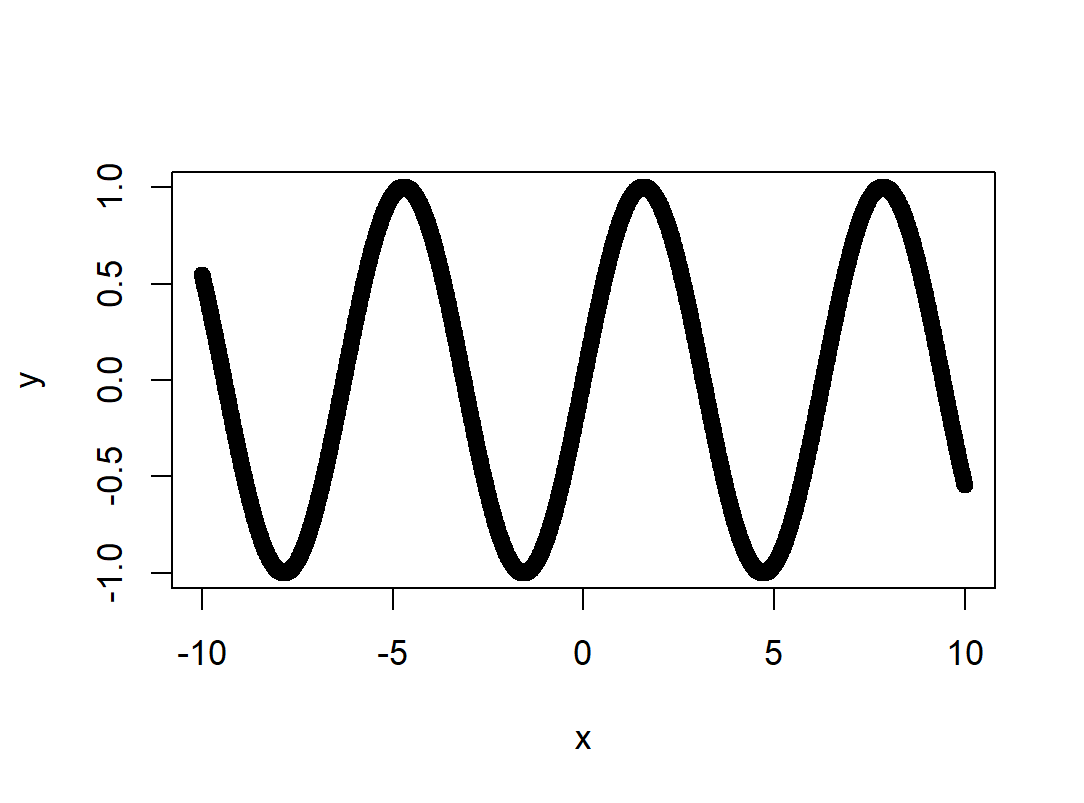
\includegraphics[width=\linewidth,trim={0 0 0 2cm},clip]{images/sinus_plot_3.png}
\end{center}
\end{minipage}


\newpage
\subsection{Argumento \texttt{type} - Tipo de representación}

El argumento \texttt{type} permite modificar el tipo de representación. Sus posibles valores son:
\begin{itemize}
	\item \texttt{"p"}: para representación con puntos.
	\item \texttt{"l"}: para representación con líneas.
	\item \texttt{"b"}: para representación con ambos, esto es, puntos unidos mediante líneas.
\end{itemize}
El tipo \texttt{"p"} es el que se dibuja por defecto. Los otros tipos se muestran a continuación:

\bigskip

\begin{minipage}{0.45\linewidth}
\begin{lstlisting}[style=rstyle]
x <- seq(-10, 10, by=0.5)
y <- sin(x)
plot(x, y, type = "l")
\end{lstlisting}
\begin{center}
	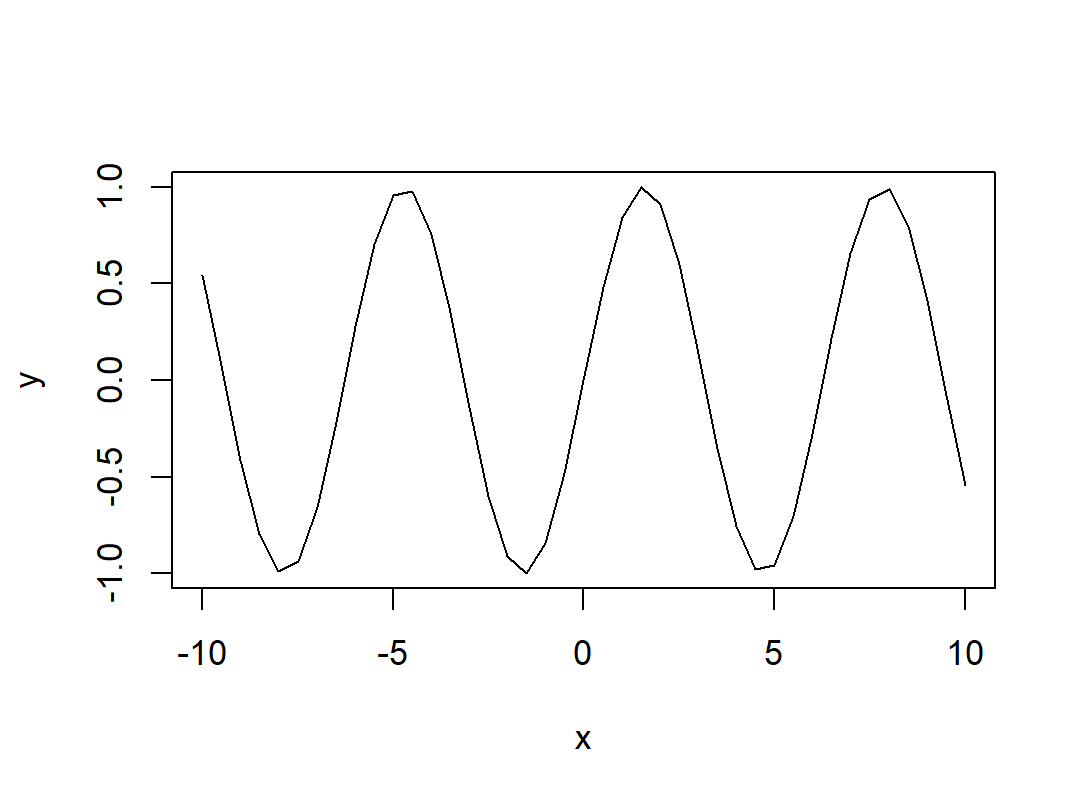
\includegraphics[width=\linewidth,trim={0 0 0 2cm},clip]{images/plot_type_l.png}
\end{center}
\end{minipage}
~
\hspace{0.5cm}
~
\begin{minipage}{0.45\textwidth}
\begin{lstlisting}[style=rstyle]
x <- seq(-10, 10, by=0.5)
y <- sin(x)
plot(x, y, type = "b")
\end{lstlisting}
\begin{center}
	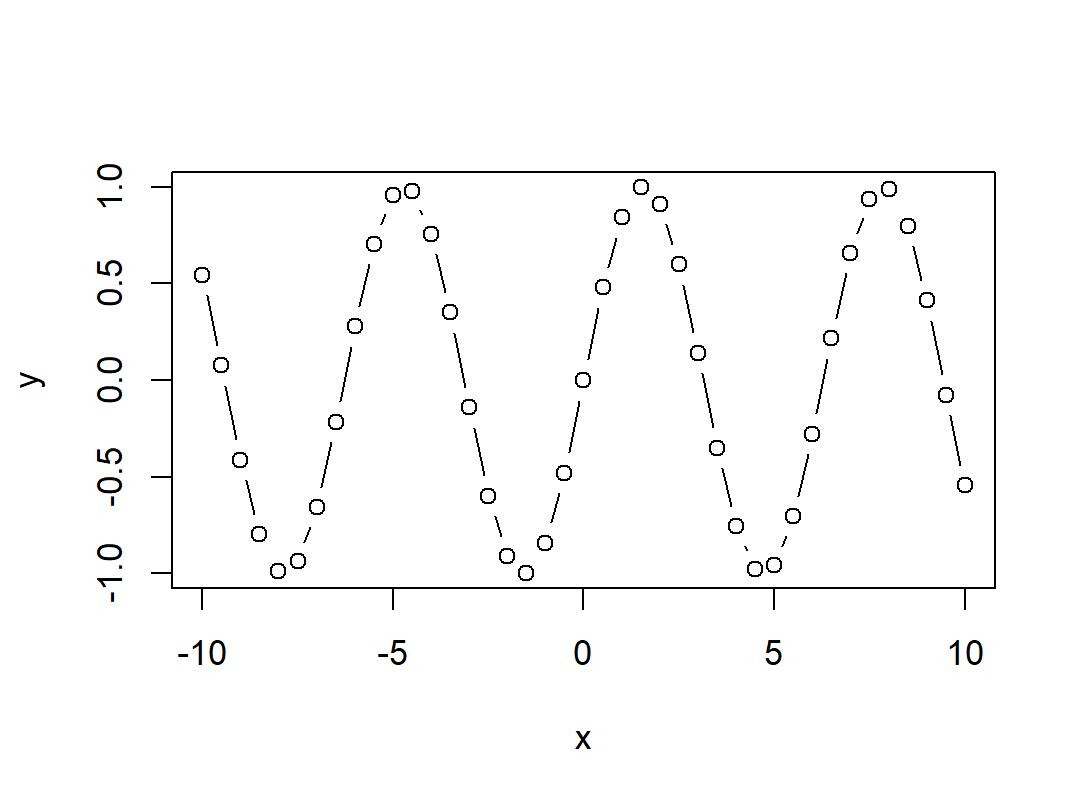
\includegraphics[width=\linewidth,trim={0 0 0 2cm},clip]{images/plot_type_b.png}
\end{center}
\end{minipage}


\subsection{Argumento \texttt{col} - Color del gráfico}

El argumento \texttt{col} permite modificar el color de la representación. Algunos de los valores más habituales son:
\begin{center}
	\begin{tabular}{ccccccc}
		\textcolor{gray}{\texttt{"white"}}
		& \textcolor{black}{\texttt{"black"}}
		& \textcolor{blue}{\texttt{"blue"}}		
		& \textcolor{brown}{\texttt{"brown"}}
		& \textcolor{cyan}{\texttt{\textquotedblleft cyan"}} 
		& \textcolor{DarkGreen}{\texttt{"darkgreen"}}
		& \textcolor{gray}{\texttt{"gray"}} \\
		\textcolor{green}{\texttt{"green"}}
		& \textcolor{magenta}{\texttt{"magenta"}}		
		& \textcolor{orange}{\texttt{\textquotedblleft orange"}} 
		& \textcolor{pink}{\texttt{"pink"}}
		& \textcolor{purple}{\texttt{\textquotedblleft purple"}}
		& \textcolor{red}{\texttt{\textquotedblleft red"}}
		& \textcolor{DarkYellow}{\texttt{\textquotedblleft yellow"}}
	\end{tabular}
\end{center}
Podemos ver una lista completa de los colores predefinidos que podemos especificar mediante una cadena de texto con el comando:
\begin{lstlisting}[style=rconsole]
> colors()
\end{lstlisting}

\bigskip

\begin{minipage}{0.45\linewidth}
\begin{lstlisting}[style=rstyle]
x <- seq(-10, 10, by=0.1)
y <- sin(x)
plot(x,y,type="l",col="red")
\end{lstlisting}
\begin{center}
	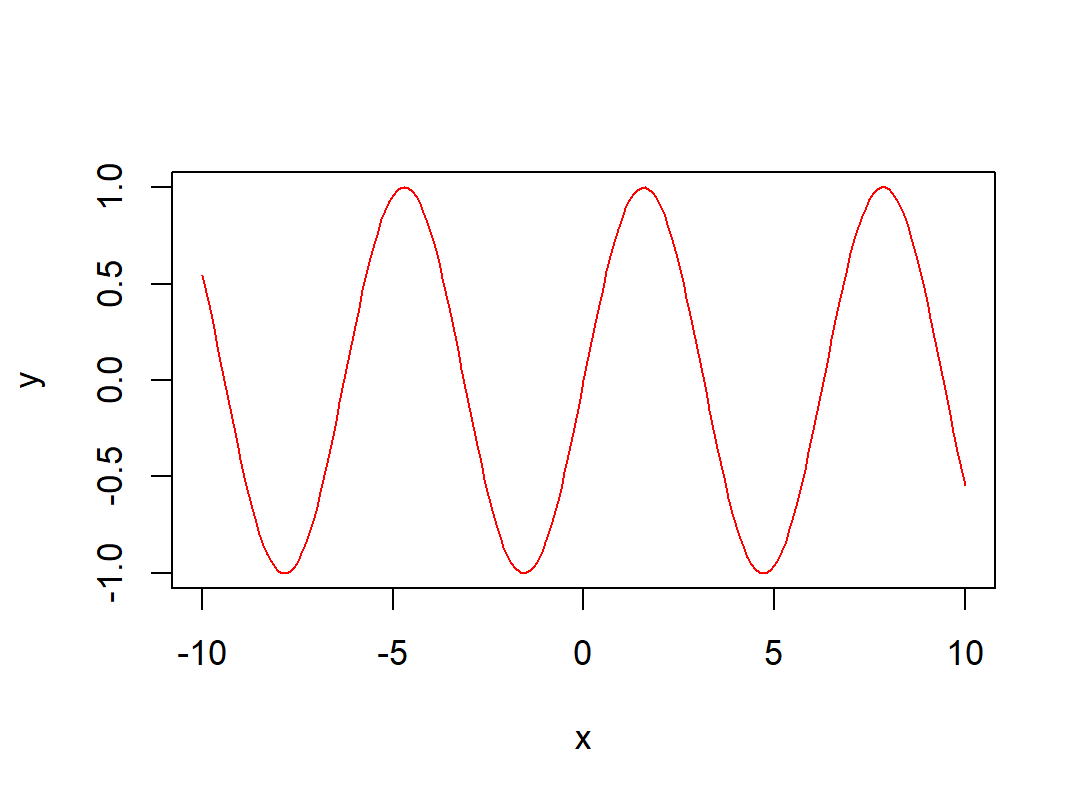
\includegraphics[width=\linewidth,trim={0 0 0 2cm},clip]{images/plot_col_1.png}
\end{center}
\end{minipage}
~
\hspace{0.5cm}
~
\begin{minipage}{0.45\textwidth}
\begin{lstlisting}[style=rstyle]
x <- seq(-10, 10, by=0.1)
y <- sin(x)
plot(x,y,type="p",col="cyan")
\end{lstlisting}
\begin{center}
	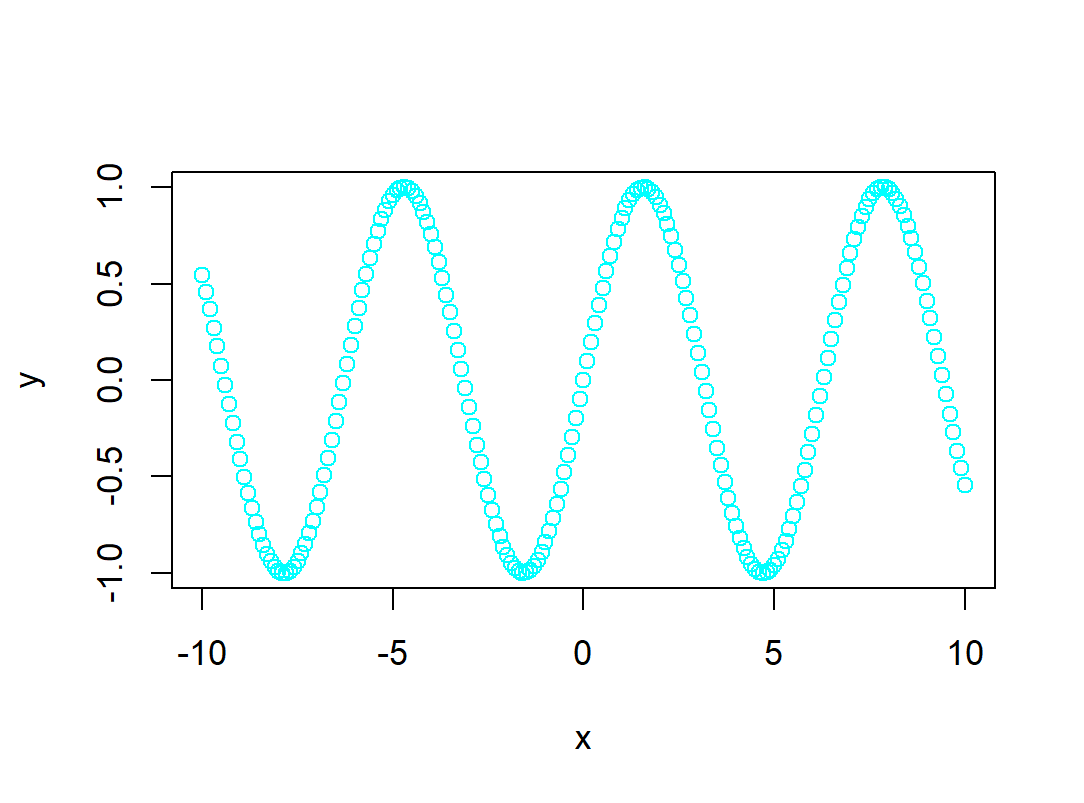
\includegraphics[width=\linewidth,trim={0 0 0 2cm},clip]{images/plot_col_2.png}
\end{center}
\end{minipage}

Si damos un vector de colores, entonces los puntos se colorearán de forma alternada de esos colores.

\begin{lstlisting}[style=rstyle]
x <- seq(-10, 10, by=0.25)
y <- sin(x)
plot(x,y,type = "p",
         col = c("green","darkgreen","black","blue","cyan","green",
                 "yellow","orange","red","pink","purple"))
\end{lstlisting}
\begin{center}
	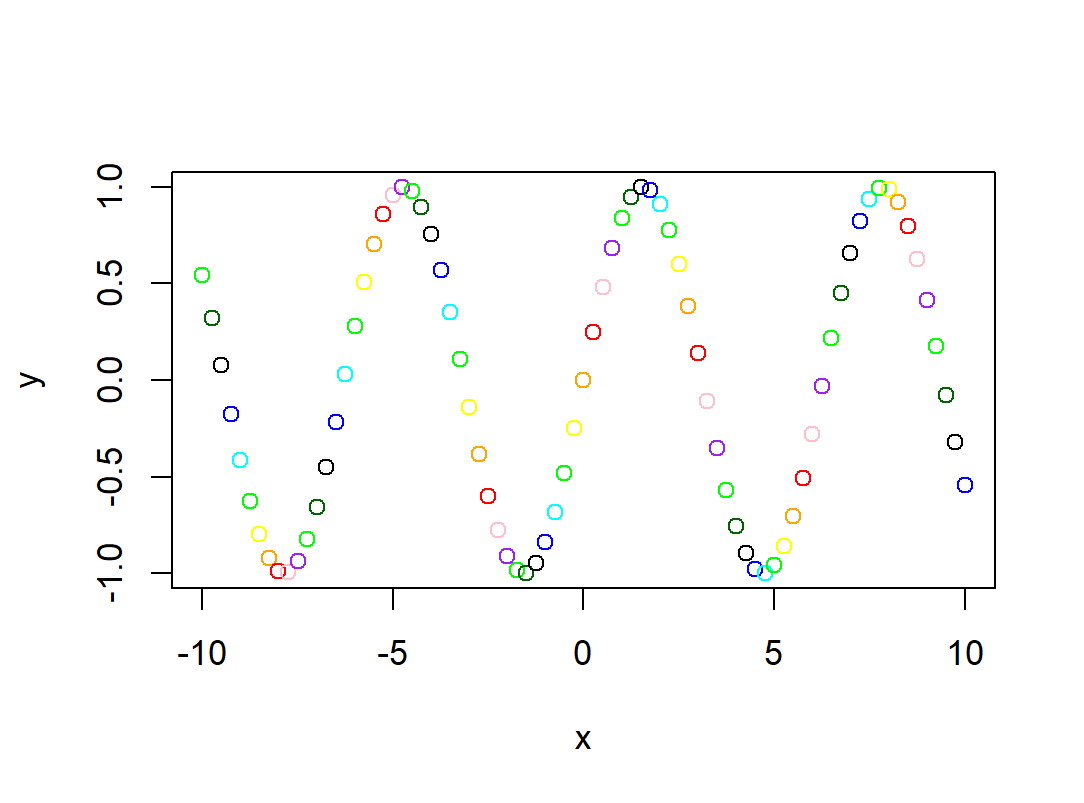
\includegraphics[width=0.75\linewidth,trim={0 0.5cm 0 1.5cm},clip]{images/plot_col_3.png}
\end{center}





\subsection{Argumentos \texttt{main}, \texttt{xlab} y \texttt{ylab} - Título y etiquetas en los ejes}


El argumento \texttt{main} permite poner título al gráfico. Los argumentos \texttt{xlab} e \texttt{ylab} permiten cambiar el nombre a los ejes.

\begin{lstlisting}[style=rstyle]
x <- seq(-10, 10, by=0.1)
y <- sin(x)
plot(x,y,type = "p",
         col = "cyan",
         main = "Gráfica de sin(x)",
         xlab = "Eje de la variable independiente x",
         ylab = "Eje de la variable dependiente y")
\end{lstlisting}
\begin{center}
	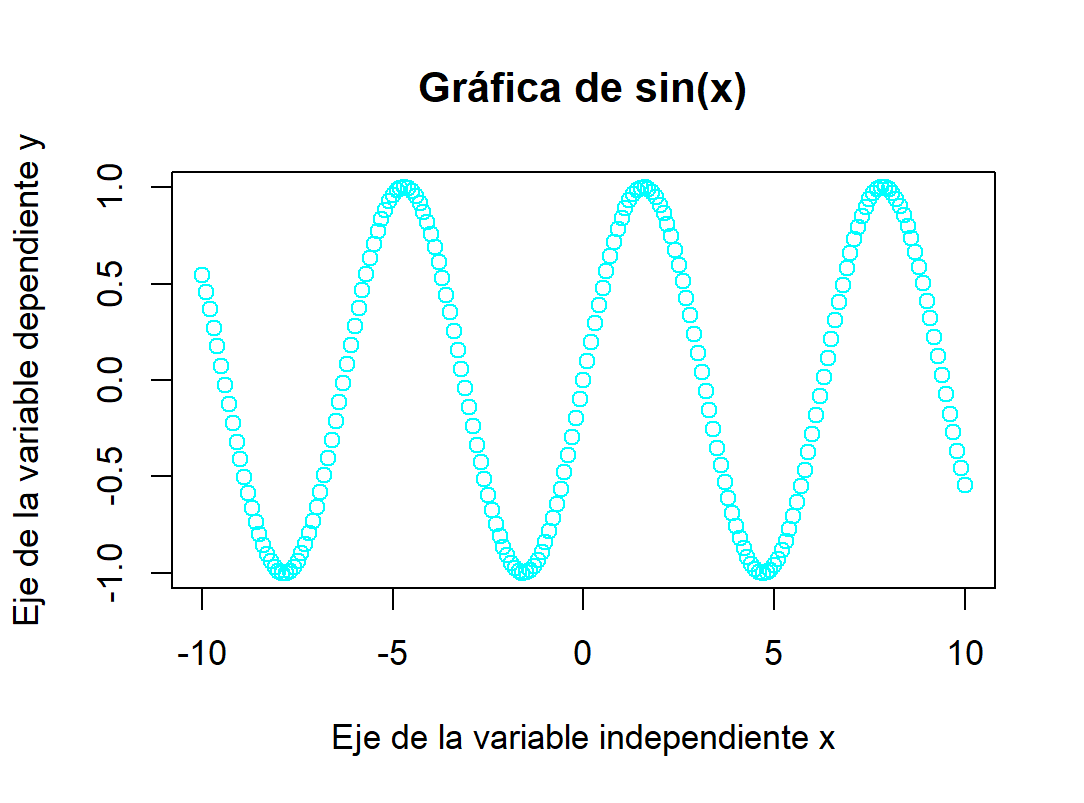
\includegraphics[width=0.75\linewidth,trim={0 0.5cm 0 0},clip]{images/plot_title.png}
\end{center}



\subsection{Argumento \texttt{pch} - Tipo de punto}

El tipo de punto se puede especificar con el argumento \texttt{pch} (\emph{plotting character}). Podemos asignarle un número entre el 1 y el 25. En ese caso, el tipo de punto viene dado por:
\begin{figure}[H]
	\centering
	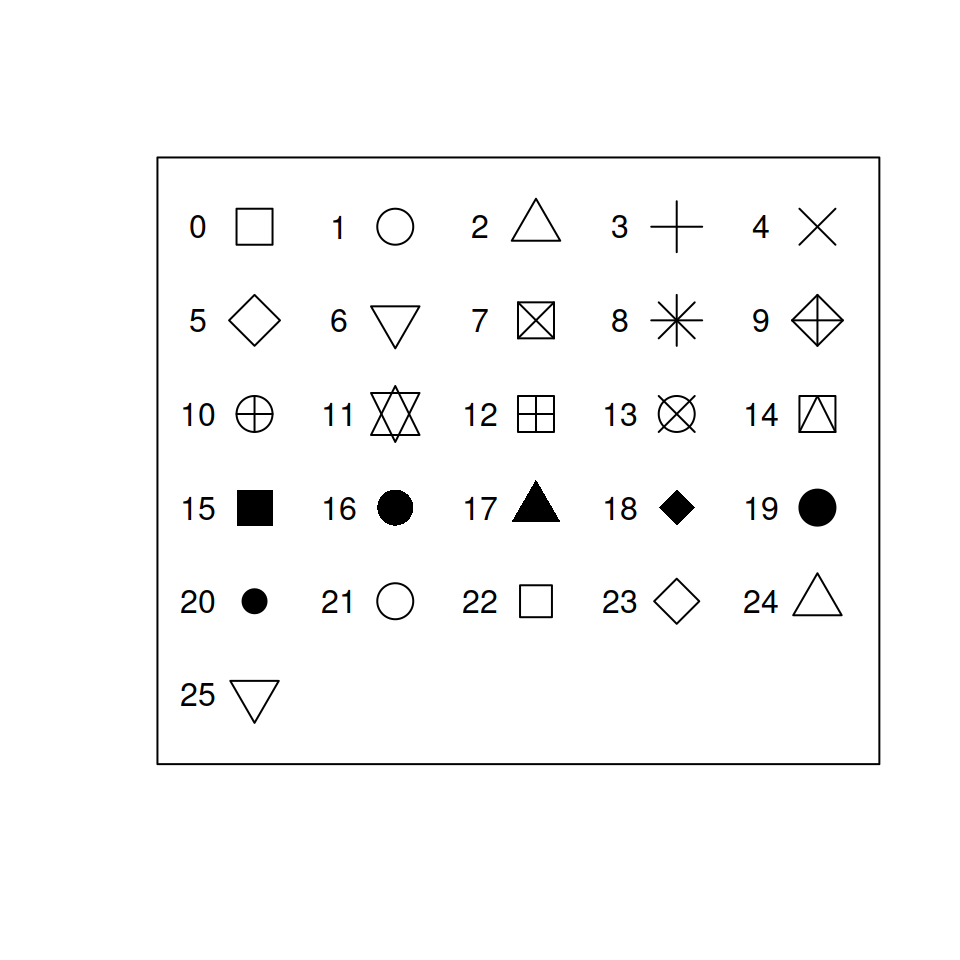
\includegraphics[width=0.4\linewidth,trim={0 2.1cm 0 0.85cm}]{images/pch-symbols}
	\caption{Imagen obtenida de \url{https://r-charts.com/base-r/pch-symbols/}}
\end{figure}

También podemos especificar una lista de valores para indicar que se alternan ciertos símbolos, o incluso podemos especificar una letra para que sea el símbolo del punto.

\bigskip

\noindent
\begin{minipage}{0.45\linewidth}
\begin{lstlisting}[style=rstyle]
x <- seq(-10, 10, by=0.25)
y <- sin(x)
plot(x,y,type="p",
  col="brown", main="sin(x)",
  xlab="Eje x", ylab="Eje y",
  pch=10)
\end{lstlisting}
\begin{center}
	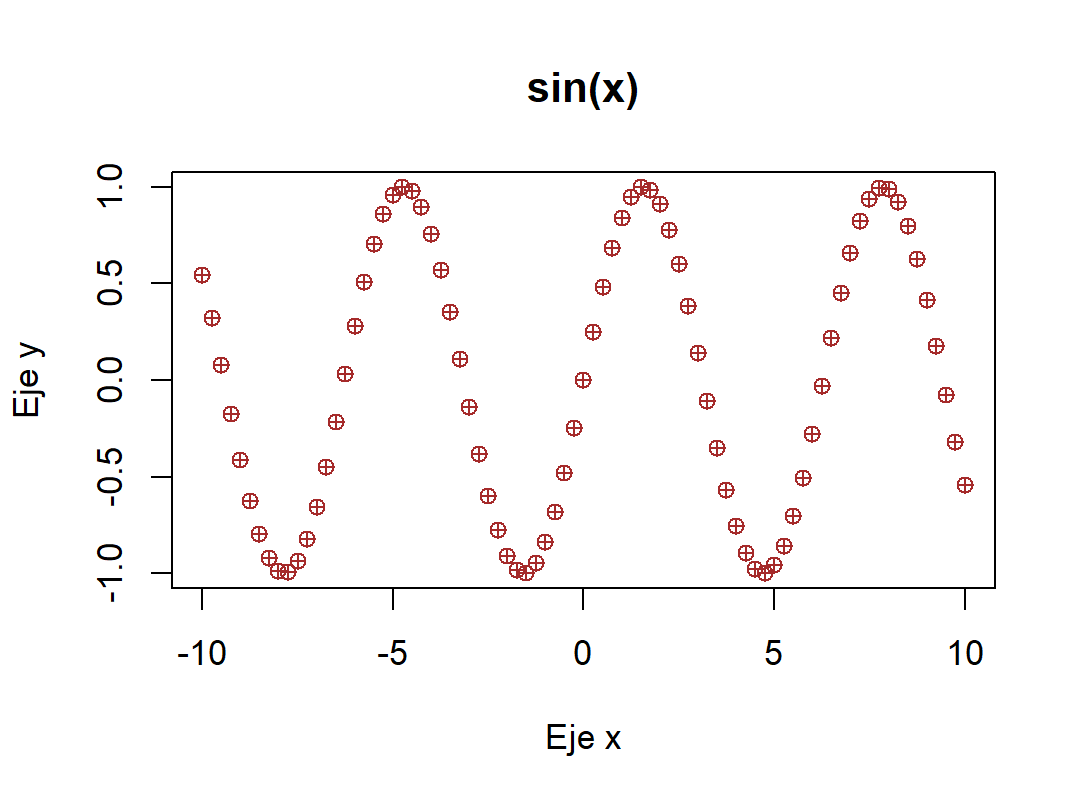
\includegraphics[width=\linewidth,trim={0 0 0 2cm},clip]{images/plot_pch_1.png}
\end{center}
\end{minipage}
~
\hspace{0.5cm}
~
\begin{minipage}{0.45\textwidth}
\begin{lstlisting}[style=rstyle]
x <- seq(-10, 10, by=0.25)
y <- sin(x)
plot(x,y,type="p",
  col="red", main="sin(x)",
  xlab="Eje x", ylab="Eje y",
  pch=c(0,1,2,3,15,16,17,4))
\end{lstlisting}

\begin{center}
	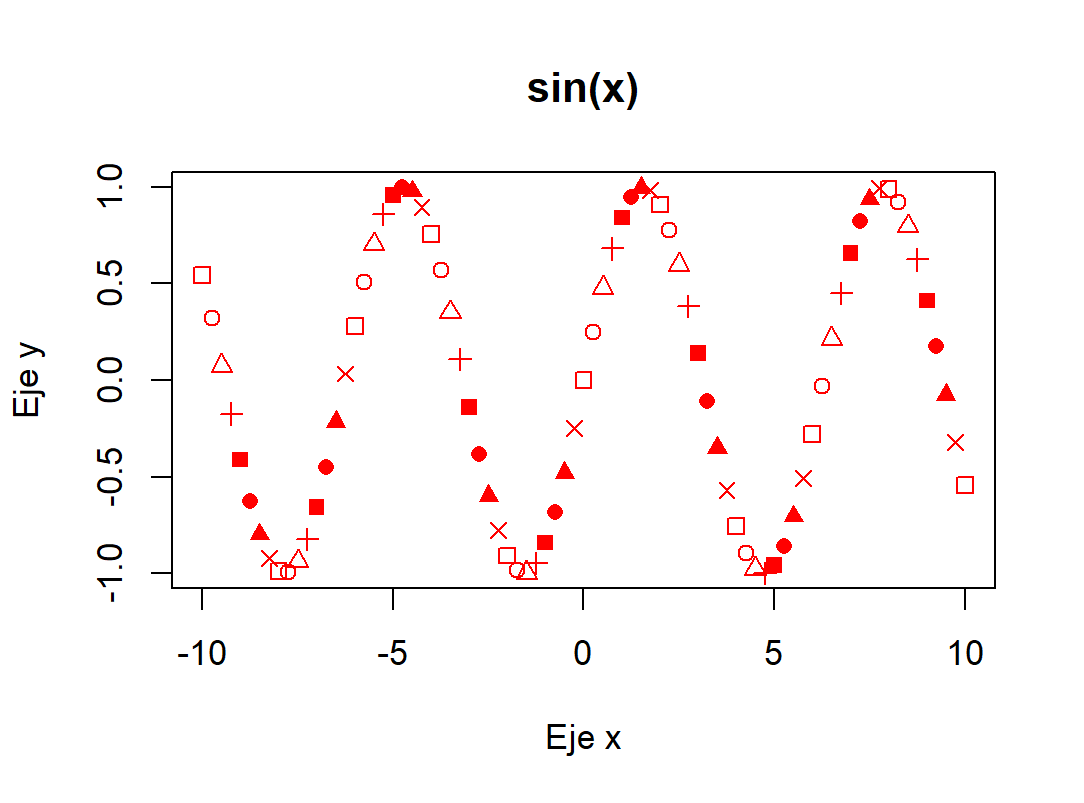
\includegraphics[width=\linewidth,trim={0 0 0 2cm},clip]{images/plot_pch_2.png}
\end{center}
\end{minipage}

\noindent
\begin{minipage}{0.45\linewidth}
\begin{lstlisting}[style=rstyle]
x <- seq(-10, 10, by=0.25)
y <- sin(x)
plot(x,y,type="p",
  col="blue", main="sin(x)",
  xlab="Eje x", ylab="Eje y",
  pch="m")
\end{lstlisting}
\begin{center}
	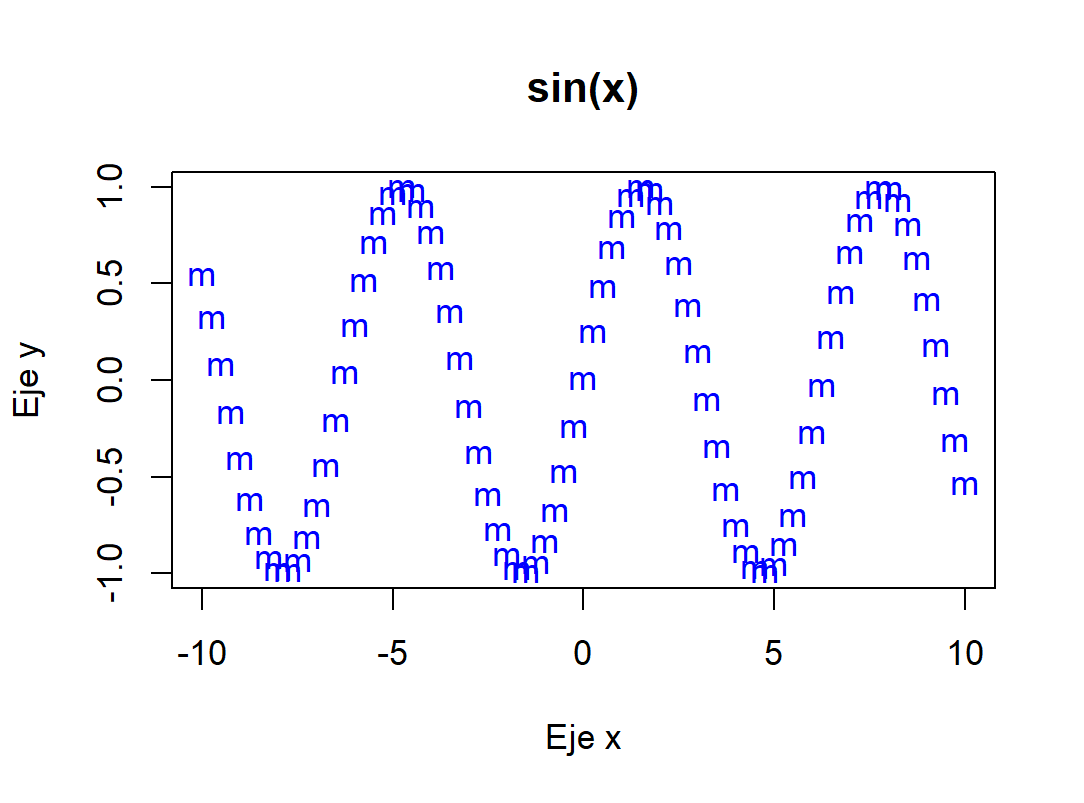
\includegraphics[width=\linewidth,trim={0 0 0 2cm},clip]{images/plot_pch_3.png}
\end{center}
\end{minipage}
~
\hspace{0.5cm}
~
\begin{minipage}{0.45\textwidth}
\begin{lstlisting}[style=rstyle]
x <- seq(-10, 10, by=0.25)
y <- sin(x)
plot(x,y,type="p",
  col="orange", main="sin(x)",
  xlab="Eje x", ylab="Eje y",
  pch=c("a","b","c","d","e"))
\end{lstlisting}

\begin{center}
	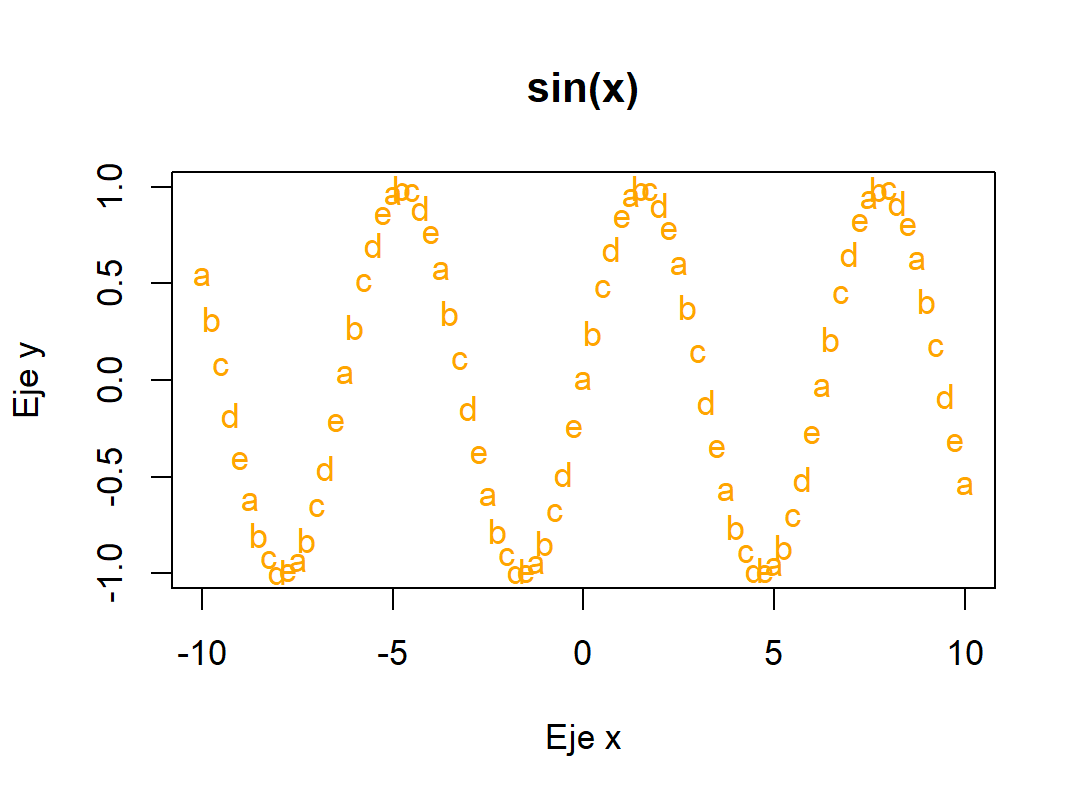
\includegraphics[width=\linewidth,trim={0 0 0 2cm},clip]{images/plot_pch_4.png}
\end{center}
\end{minipage}




\subsection{Argumento \texttt{cex} - Tamaño del punto}


Con el argumento \texttt{cex} podemos especificar el tamaño del punto. Por defecto, este tamaño es 1. Si especificamos varios valores, entonces los puntos tomarán dichos valores. 

\bigskip

\noindent
\begin{minipage}{0.45\linewidth}
\begin{lstlisting}[style=rstyle]
x <- seq(-10, 10, by=0.25)
y <- sin(x)
plot(x,y,type = "p",
         col = "green",
         main = "sin(x)",
         xlab = "Eje x",
         ylab = "Eje y",
         pch = 9,
         cex = 0.5)
\end{lstlisting}
\begin{center}
	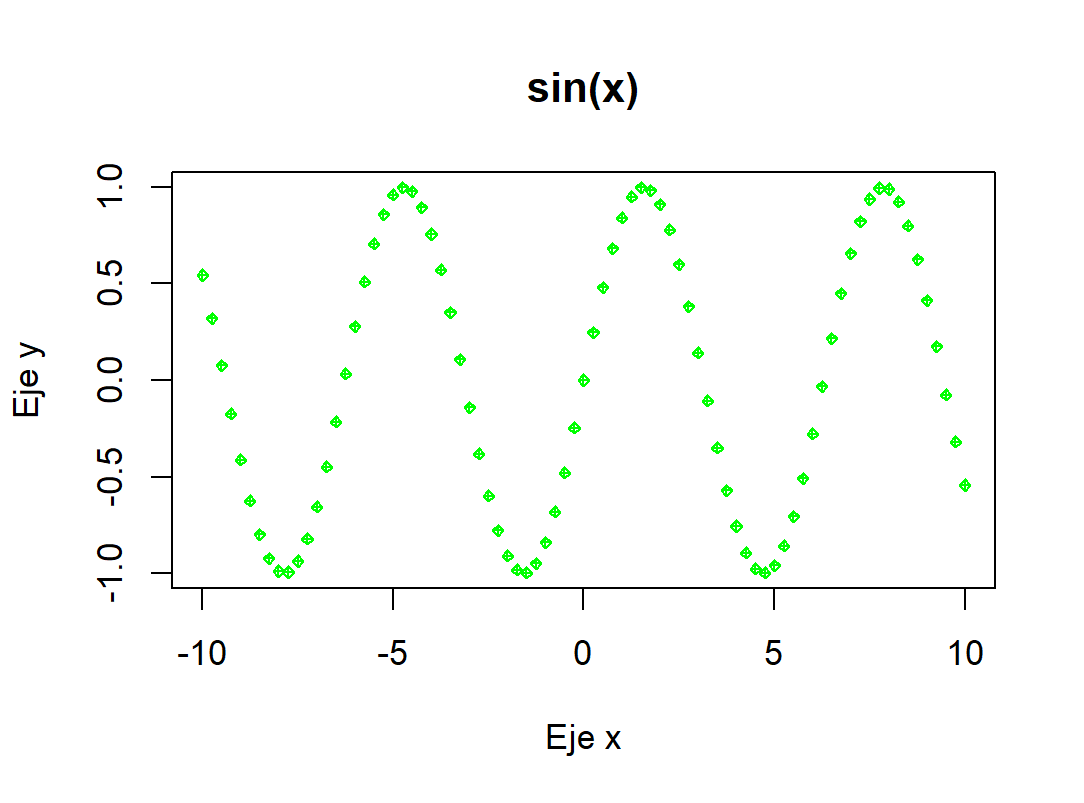
\includegraphics[width=\linewidth,trim={0 0 0 2cm},clip]{images/plot_cex_1.png}
\end{center}
\end{minipage}
~
\hspace{0.5cm}
~
\begin{minipage}{0.45\textwidth}
\begin{lstlisting}[style=rstyle]
x <- seq(-10, 10, by=0.25)
y <- sin(x)
plot(x,y,type = "p",
         col = "green",
         main = "sin(x)",
         xlab = "Eje x",
         ylab = "Eje y",
         pch = 9,
         cex = 1)
\end{lstlisting}

\begin{center}
	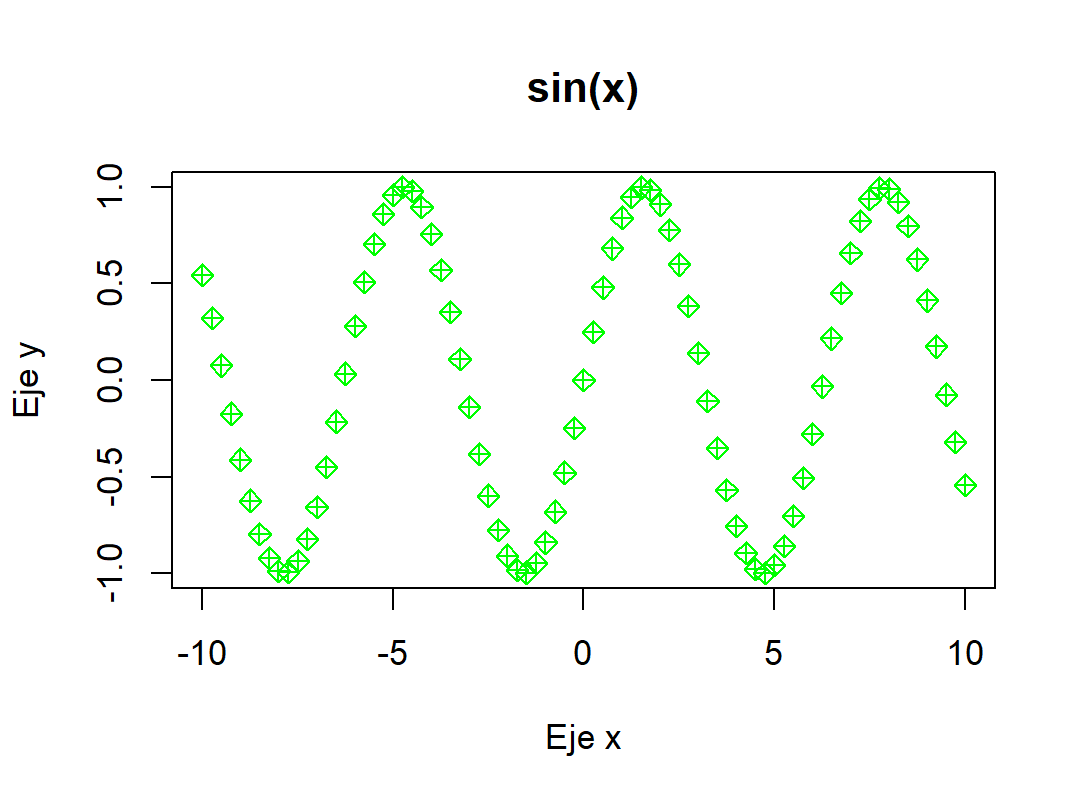
\includegraphics[width=\linewidth,trim={0 0 0 2cm},clip]{images/plot_cex_2.png}
\end{center}
\end{minipage}

\noindent
\begin{minipage}{0.45\linewidth}
\begin{lstlisting}[style=rstyle]
x <- seq(-10, 10, by=0.25)
y <- sin(x)
plot(x,y,type = "p",
         col = "green",
         main = "sin(x)",
         xlab = "Eje x",
         ylab = "Eje y",
         pch = 9,
         cex = 2)
\end{lstlisting}
\begin{center}
	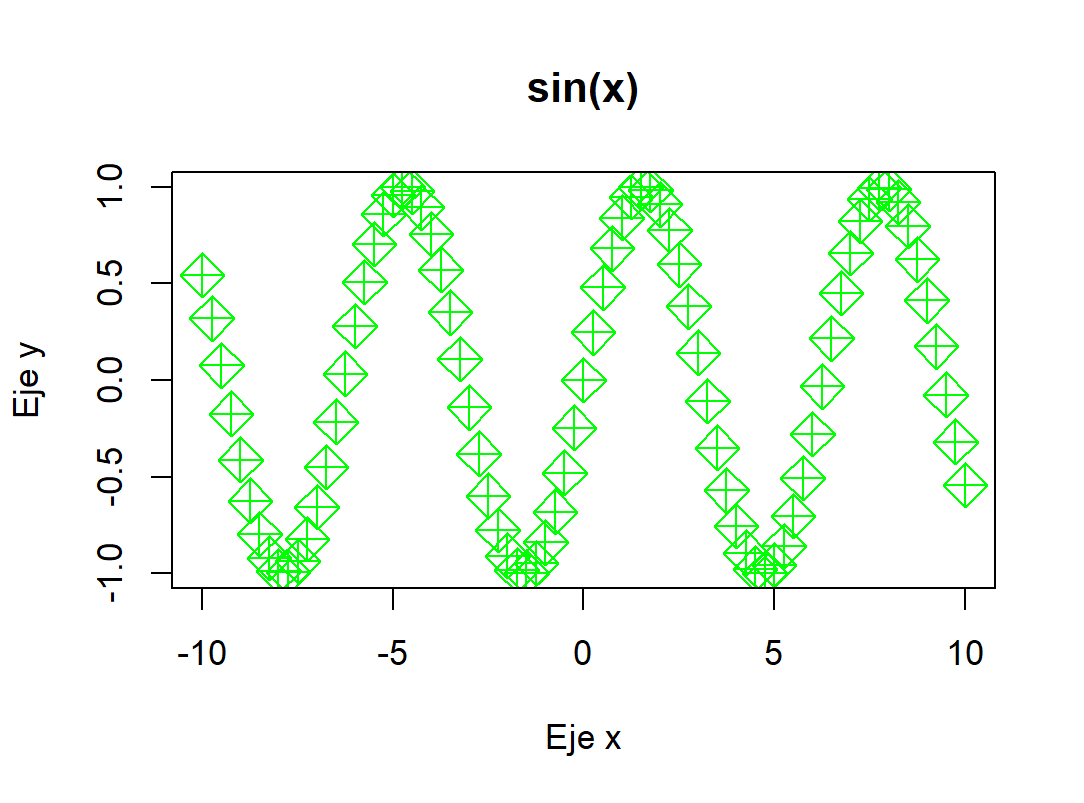
\includegraphics[width=\linewidth,trim={0 0 0 2cm},clip]{images/plot_cex_3.png}
\end{center}
\end{minipage}
~
\hspace{0.5cm}
~
\begin{minipage}{0.45\textwidth}
\begin{lstlisting}[style=rstyle]
x <- seq(-10, 10, by=0.25)
y <- sin(x)
plot(x,y,type = "p",
         col = "green",
         main = "sin(x)",
         xlab = "Eje x",
         ylab = "Eje y",
         pch = 9,
         cex = seq(0,1,by=0.1))
\end{lstlisting}

\begin{center}
	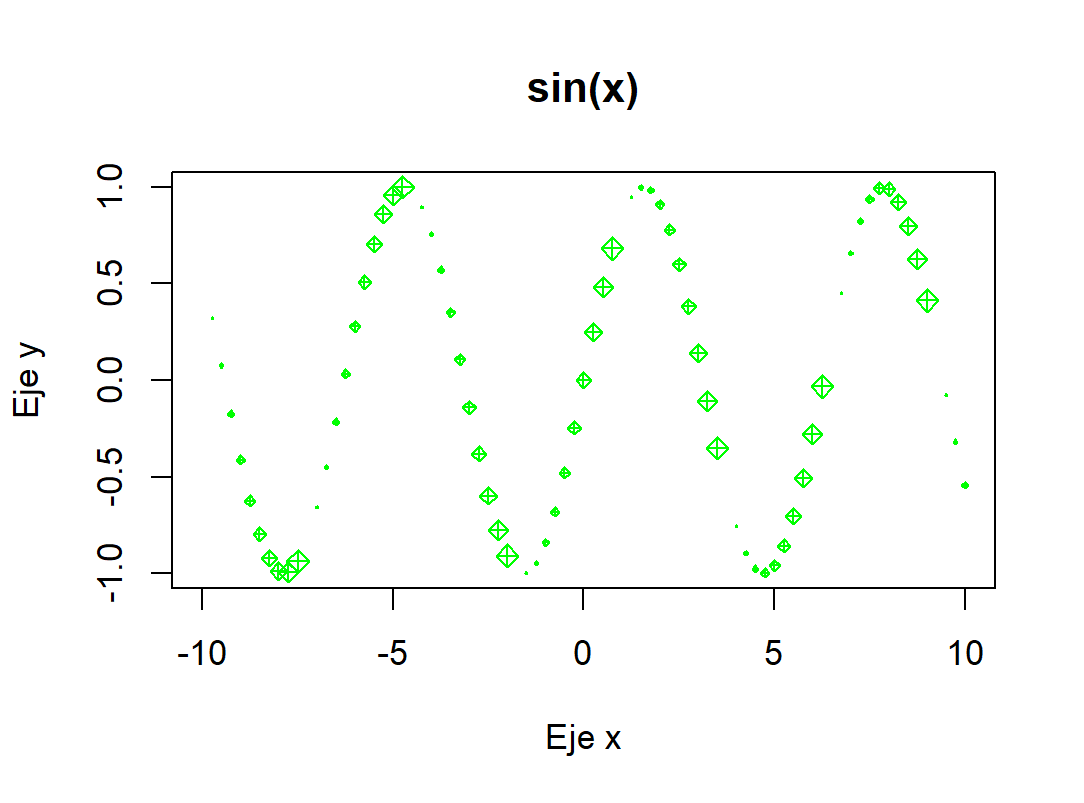
\includegraphics[width=\linewidth,trim={0 0 0 2cm},clip]{images/plot_cex_4.png}
\end{center}
\end{minipage}




\newpage
\subsection{Argumento \texttt{lty} - Tipo de línea}

Podemos especificar el tipo de línea con el argumento \texttt{lty} (\emph{line type}).
\begin{figure}[H]
	\centering
	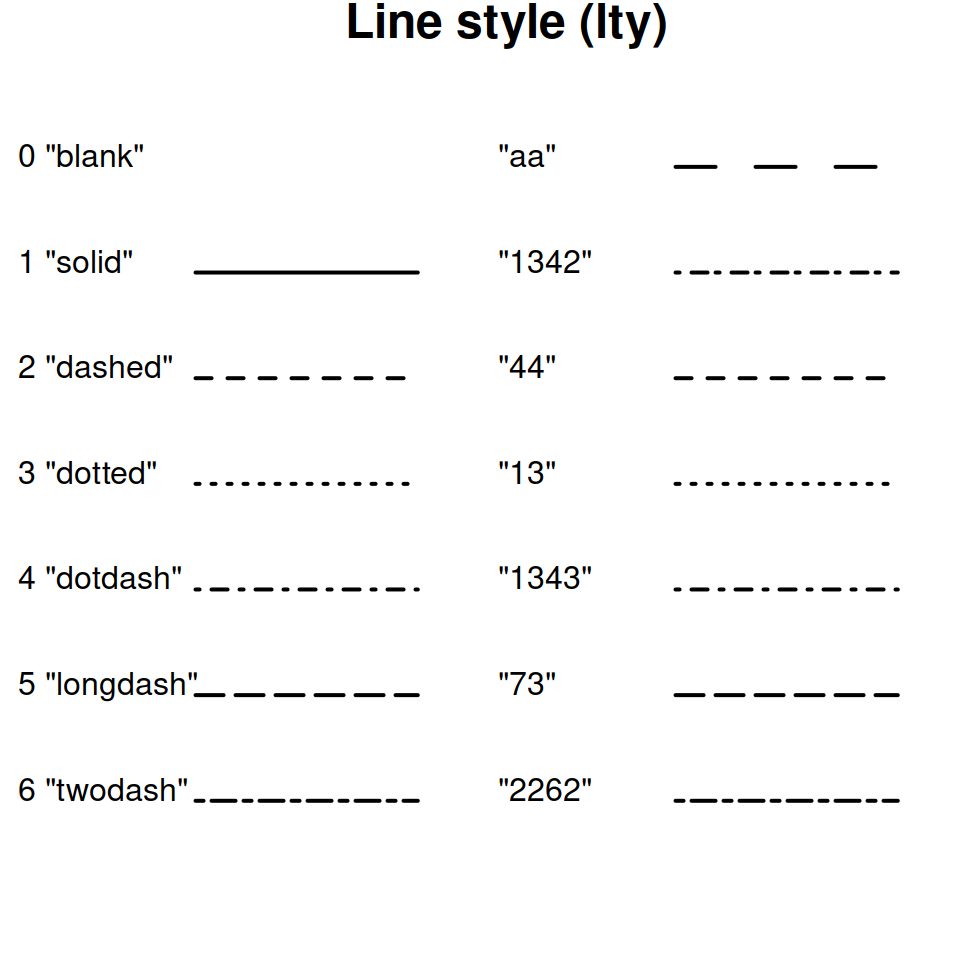
\includegraphics[width=0.4\linewidth]{images/line-types}
	\caption{Imagen obtenida de \url{https://r-charts.com/base-r/line-types/}}
\end{figure}

\bigskip

\noindent
\begin{minipage}{0.45\linewidth}
\begin{lstlisting}[style=rstyle]
x <- seq(-10, 10, by=0.25)
y <- sin(x)
plot(x,y,type = "l",
         col = "purple",
         lty = 1)
\end{lstlisting}
\begin{center}
	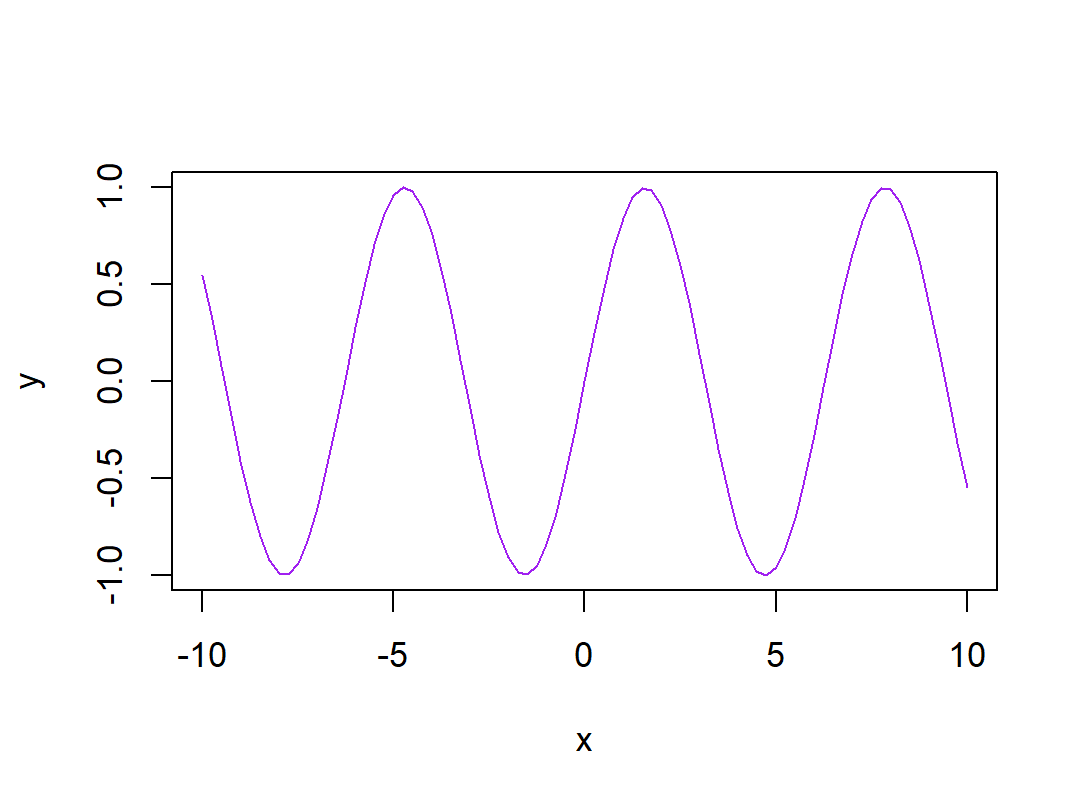
\includegraphics[width=\linewidth,trim={0 0 0 2cm},clip]{images/plot_lty_1.png}
\end{center}
\end{minipage}
~
\hspace{0.5cm}
~
\begin{minipage}{0.45\textwidth}
\begin{lstlisting}[style=rstyle]
x <- seq(-10, 10, by=0.25)
y <- sin(x)
plot(x,y,type = "l",
         col = "purple",
         lty = 3)
\end{lstlisting}

\begin{center}
	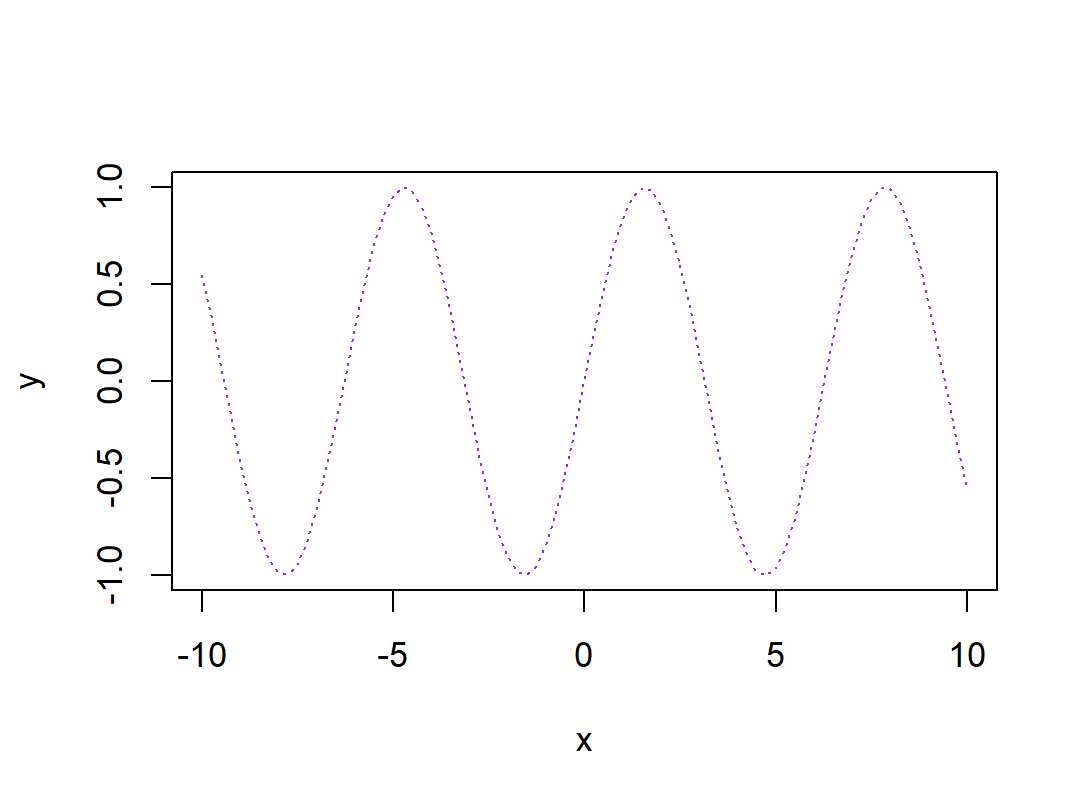
\includegraphics[width=\linewidth,trim={0 0 0 2cm},clip]{images/plot_lty_2.png}
\end{center}
\end{minipage}

\noindent
\begin{minipage}{0.45\linewidth}
\begin{lstlisting}[style=rstyle]
x <- seq(-10, 10, by=0.25)
y <- sin(x)
plot(x,y,type = "l",
         col = "purple",
         lty = 4)
\end{lstlisting}
\begin{center}
	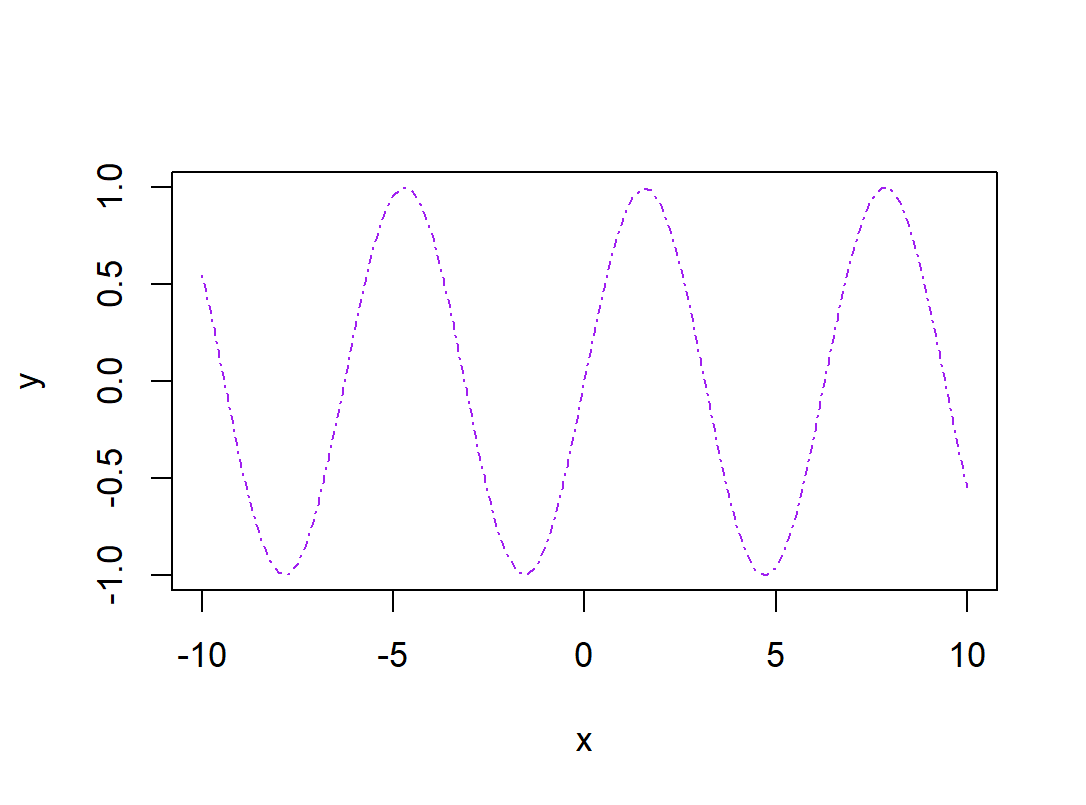
\includegraphics[width=\linewidth,trim={0 0 0 2cm},clip]{images/plot_lty_3.png}
\end{center}
\end{minipage}
~
\hspace{0.5cm}
~
\begin{minipage}{0.45\textwidth}
\begin{lstlisting}[style=rstyle]
x <- seq(-10, 10, by=0.25)
y <- sin(x)
plot(x,y,type = "l",
         col = "purple",
         lty = 5)
\end{lstlisting}

\begin{center}
	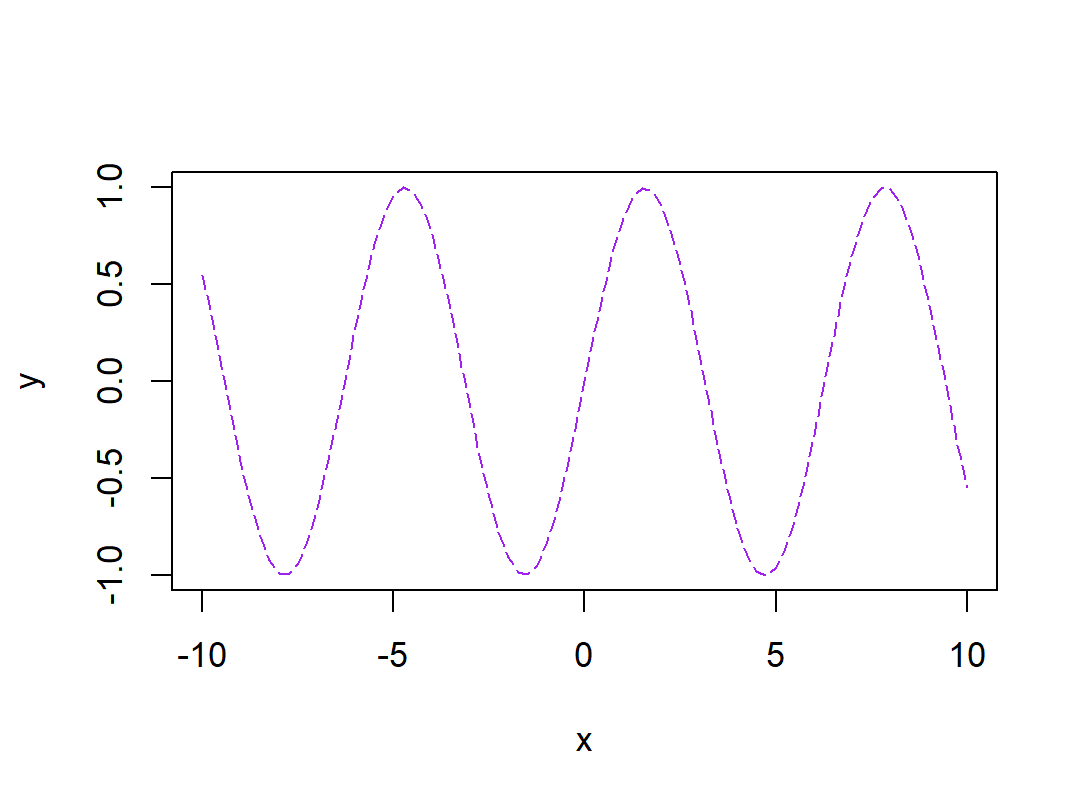
\includegraphics[width=\linewidth,trim={0 0 0 2cm},clip]{images/plot_lty_4.png}
\end{center}
\end{minipage}


\newpage
\subsection{Argumento \texttt{lwd}}

El argumento \texttt{lwd} (\emph{line width}) define el grosor de la línea del \texttt{plot()}.

\bigskip

\noindent
\begin{minipage}{0.45\linewidth}
\begin{lstlisting}[style=rstyle]
x <- seq(-10, 10, by=0.25)
y <- sin(x)
plot(x,y,type = "l",
         col = "orange",
         lwd = 0.5)
\end{lstlisting}
\begin{center}
	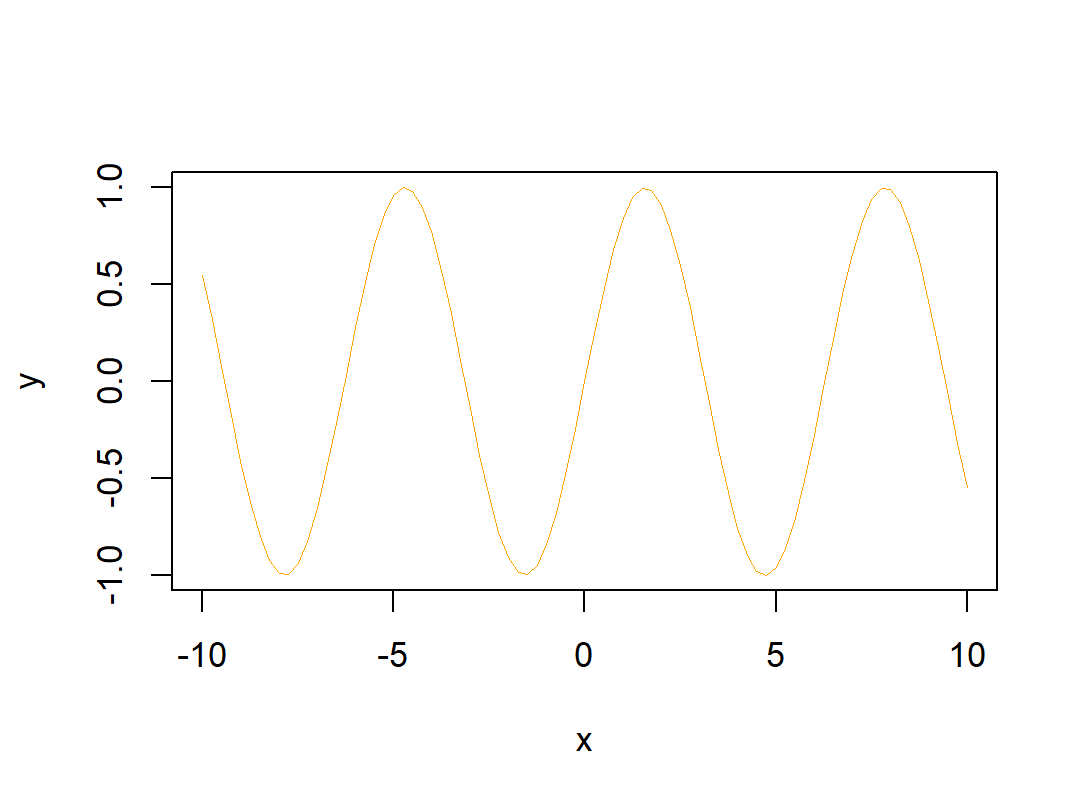
\includegraphics[width=\linewidth,trim={0 0 0 2cm},clip]{images/plot_lwd_1.png}
\end{center}
\end{minipage}
~
\hspace{0.5cm}
~
\begin{minipage}{0.45\textwidth}
\begin{lstlisting}[style=rstyle]
x <- seq(-10, 10, by=0.25)
y <- sin(x)
plot(x,y,type = "l",
         col = "orange",
         lwd = 1)
\end{lstlisting}

\begin{center}
	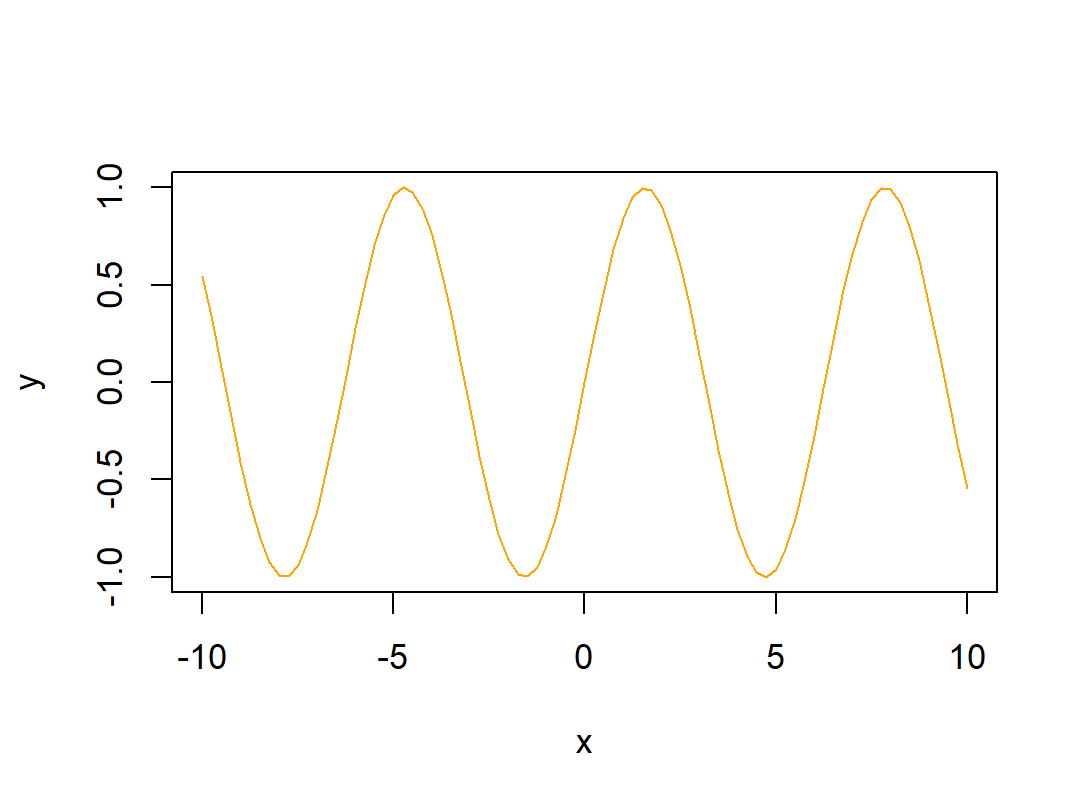
\includegraphics[width=\linewidth,trim={0 0 0 2cm},clip]{images/plot_lwd_2.png}
\end{center}
\end{minipage}

\noindent
\begin{minipage}{0.45\linewidth}
\begin{lstlisting}[style=rstyle]
x <- seq(-10, 10, by=0.25)
y <- sin(x)
plot(x,y,type = "l",
         col = "orange",
         lwd = 2)
\end{lstlisting}
\begin{center}
	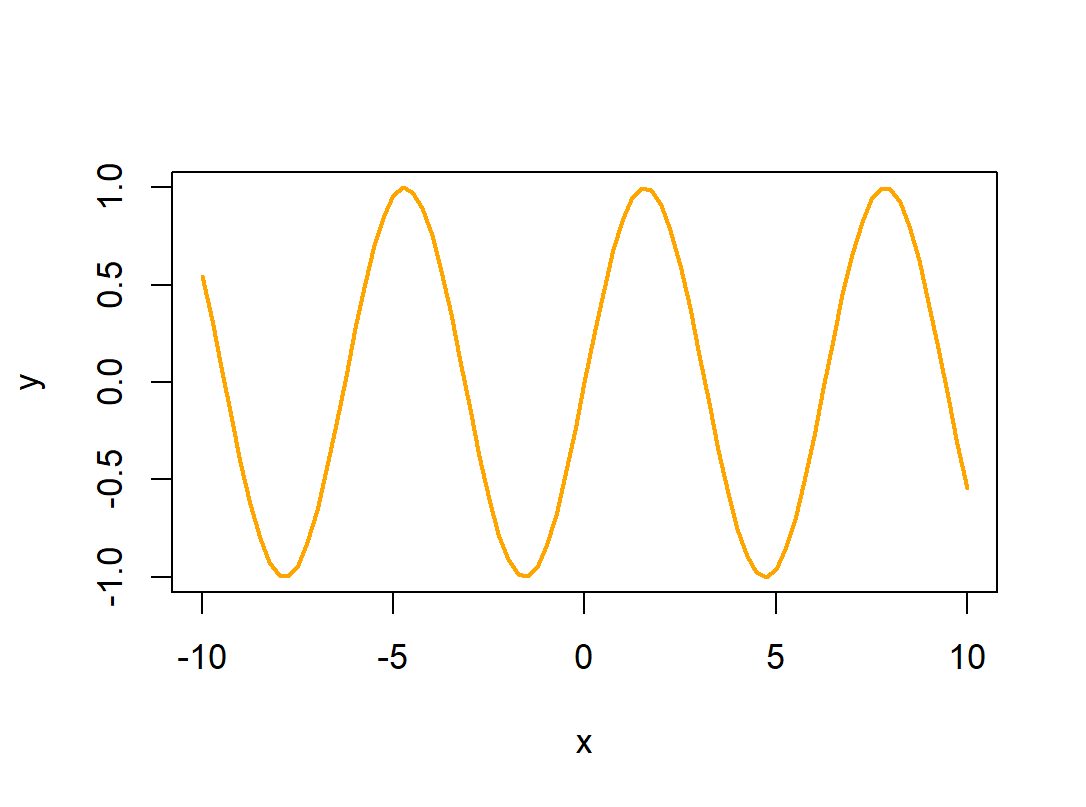
\includegraphics[width=\linewidth,trim={0 0 0 2cm},clip]{images/plot_lwd_3.png}
\end{center}
\end{minipage}
~
\hspace{0.5cm}
~
\begin{minipage}{0.45\textwidth}
\begin{lstlisting}[style=rstyle]
x <- seq(-10, 10, by=0.25)
y <- sin(x)
plot(x,y,type = "l",
         col = "orange",
         lwd = 4)
\end{lstlisting}

\begin{center}
	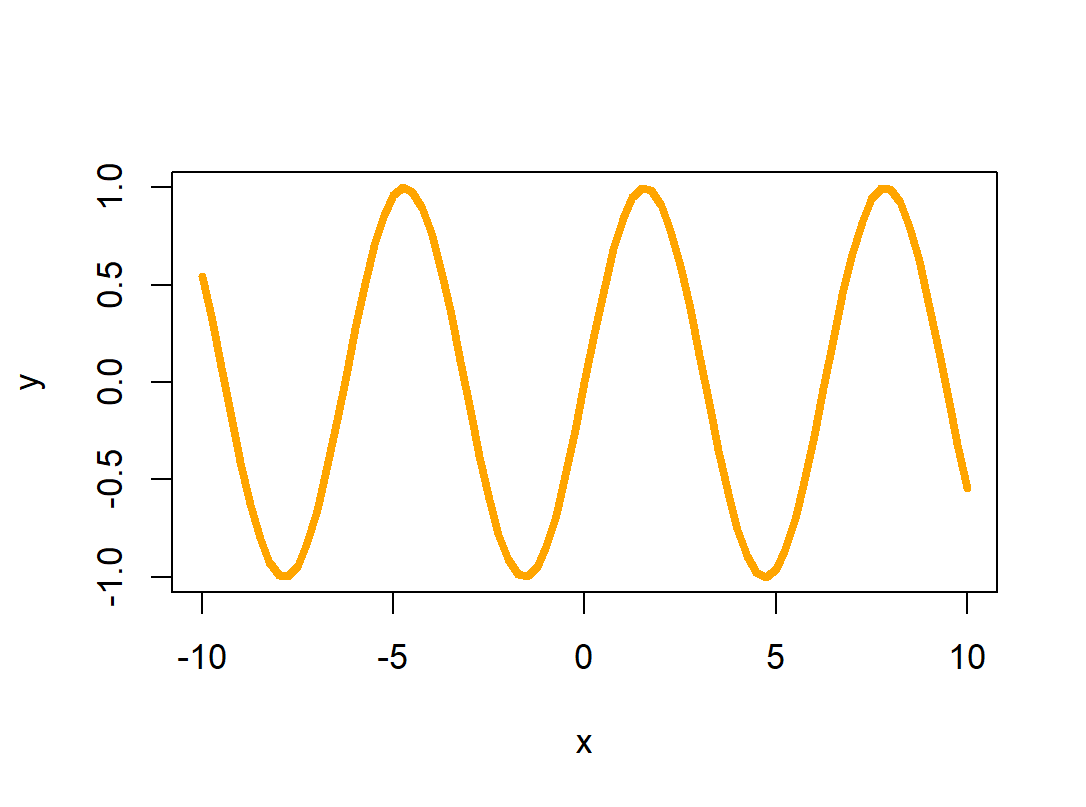
\includegraphics[width=\linewidth,trim={0 0 0 2cm},clip]{images/plot_lwd_4.png}
\end{center}
\end{minipage}






\subsection{Argumentos \texttt{xlim} e \texttt{ylim}: límites de los ejes}

Los argumentos \texttt{xlim} e \texttt{ylim} nos permiten especificar los límites del gráfico. Se especifican con un vector de dos elementos: \texttt{c(lim\_inf,lim\_sup)}.

\begin{lstlisting}[style=rstyle]
x <- seq(-10, 10, by=0.25)
y <- sin(x)
plot(x,y,type = "l",
     col = "blue",
     lwd = 2,
     xlim = c(-10,30),
     ylim = c(-1,3))
\end{lstlisting}


\begin{center}
	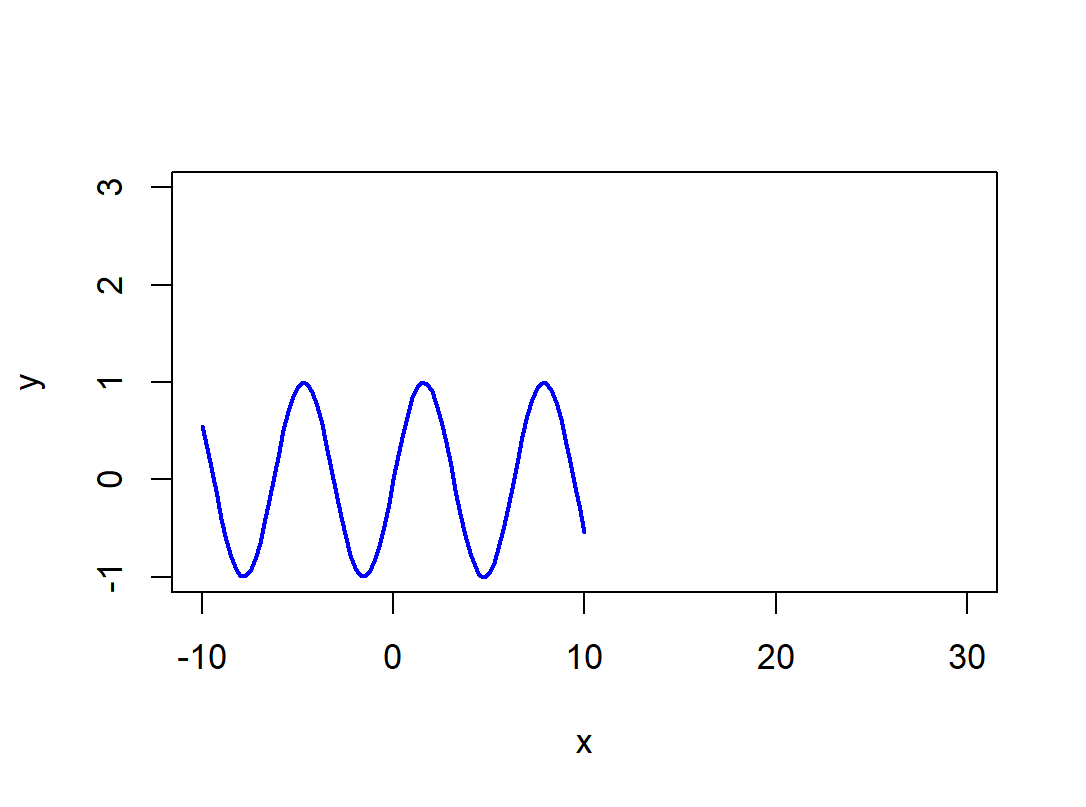
\includegraphics[width=0.75\linewidth,trim={0 0 0 2cm},clip]{images/plot_lims_0.png}
\end{center}

Observa que no se pintarán puntos que no se han especificado. Estos argumentos nos sirven para poder enfocar la región que nos interesa del gráfico.

\bigskip

\noindent
\begin{minipage}{0.45\linewidth}
\begin{lstlisting}[style=rstyle]
x <- seq(-35, 35, by=0.25)
y <- sin(x)
plot(x,y,type = "l",
     col = "blue", lwd = 2,
     xlim = c(-10,30),
     ylim = c(-1,3))
\end{lstlisting}
\begin{center}
	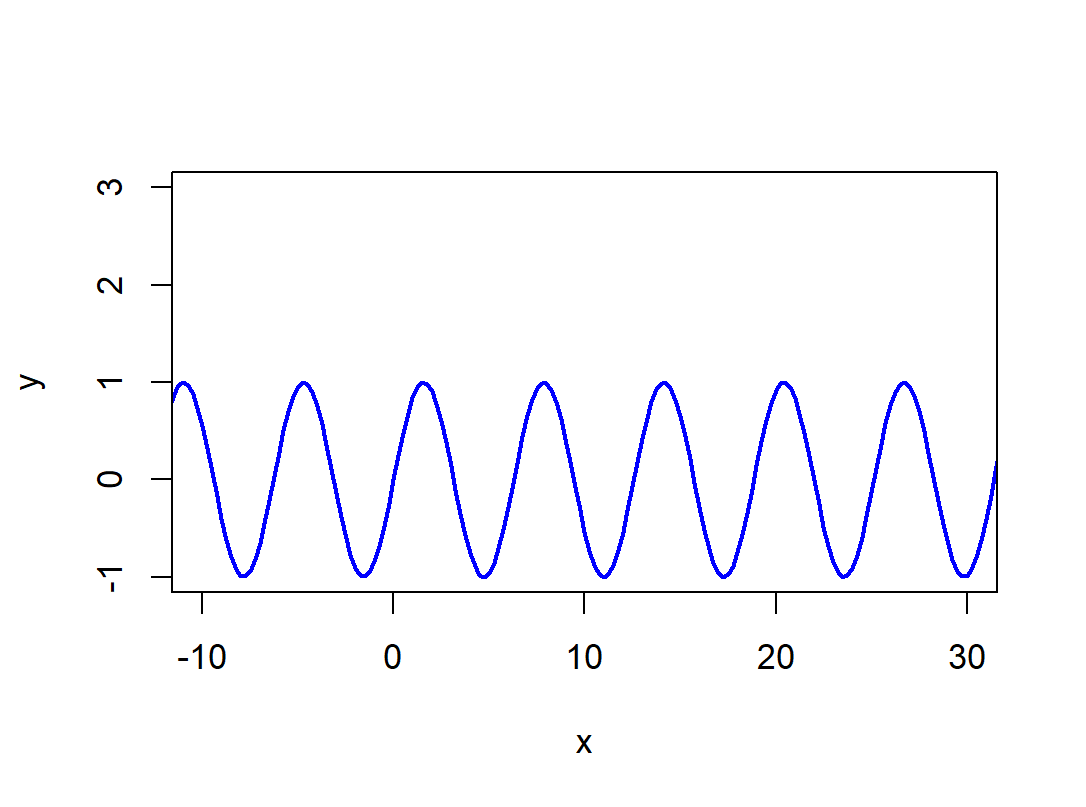
\includegraphics[width=\linewidth,trim={0 0 0 2cm},clip]{images/plot_lims_1.png}
\end{center}
\end{minipage}
~
\hspace{0.5cm}
~
\begin{minipage}{0.45\textwidth}
\begin{lstlisting}[style=rstyle]
x <- seq(-35, 35, by=0.25)
y <- sin(x)
plot(x,y,type = "l",
     col = "blue", lwd = 2,
     xlim = c(-pi,pi),
     ylim = c(-1,1))
\end{lstlisting}

\begin{center}
	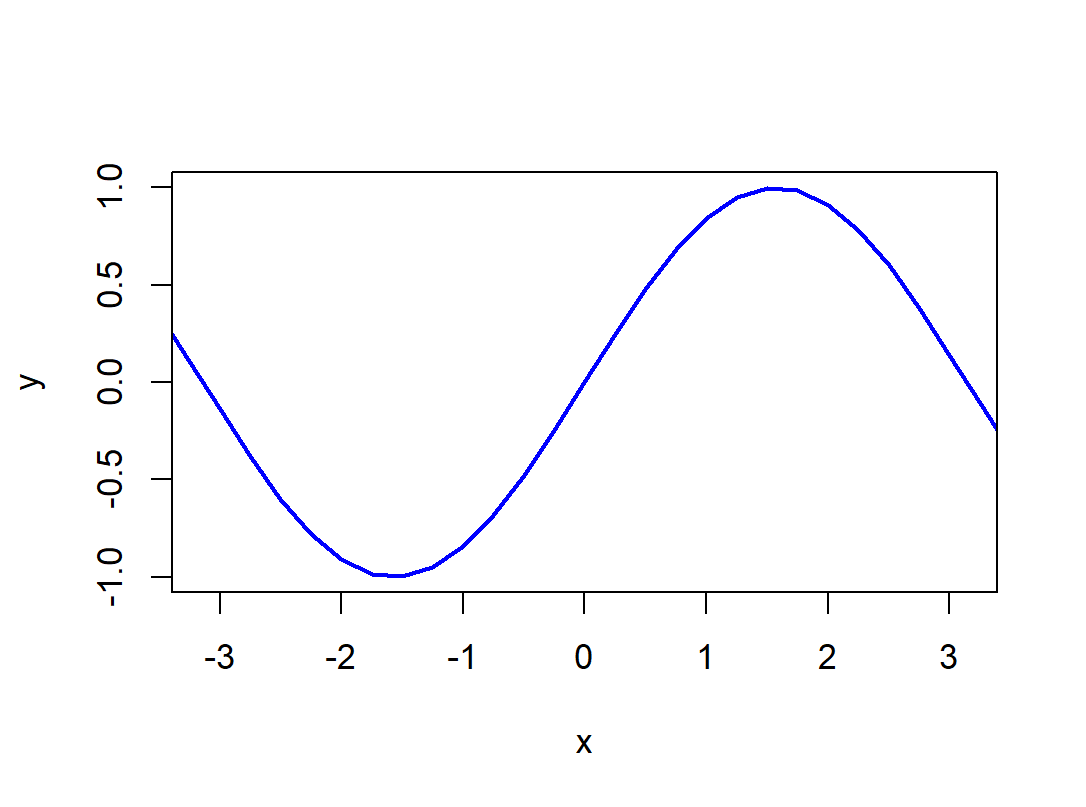
\includegraphics[width=\linewidth,trim={0 0 0 2cm},clip]{images/plot_lims_2.png}
\end{center}
\end{minipage}

\noindent
\begin{minipage}{0.45\linewidth}
\begin{lstlisting}[style=rstyle]
x <- seq(-35, 35, by=0.25)
y <- sin(x)
plot(x,y,type = "l",
     col = "blue", lwd = 2,
     xlim = c(0,pi),
     ylim = c(-1,1))
\end{lstlisting}
\begin{center}
	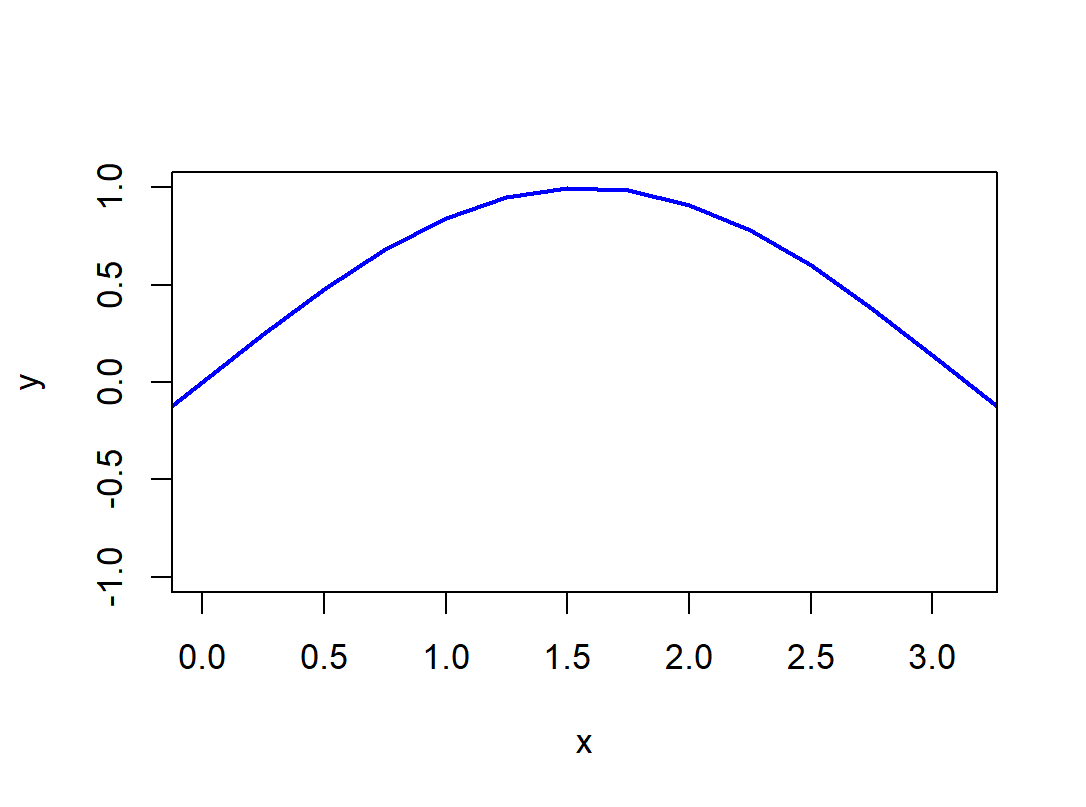
\includegraphics[width=\linewidth,trim={0 0 0 2cm},clip]{images/plot_lims_3.png}
\end{center}
\end{minipage}
~
\hspace{0.5cm}
~
\begin{minipage}{0.45\textwidth}
\begin{lstlisting}[style=rstyle]
x <- seq(-35, 35, by=0.25)
y <- sin(x)
plot(x,y,type = "l",
     col = "blue", lwd = 2,
     xlim = c(-10,10),
     ylim = c(0,2))
\end{lstlisting}

\begin{center}
	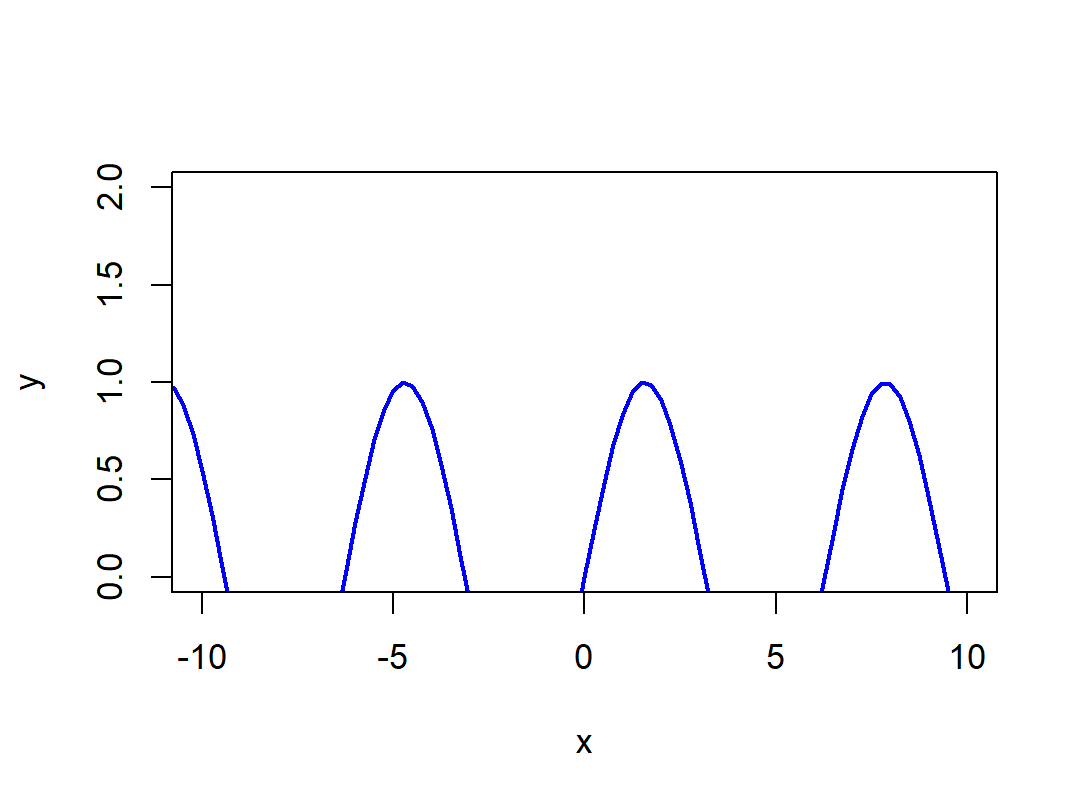
\includegraphics[width=\linewidth,trim={0 0 0 2cm},clip]{images/plot_lims_4.png}
\end{center}
\end{minipage}




\newpage
\begin{exercise} \R\ define las siguientes funciones matemáticas básicas:
\begin{center}
	\begin{tabular}{|l|l|} \hline
		\textbf{Función} & \textbf{Descripción} \\ \hline
		\verb|x^n| & Potencia $n$-ésima de $x$ \\
		\texttt{sqrt(x)} & Función raíz cuadrada \\
		\texttt{exp(x)} & Función exponencial \\
		\texttt{log(x)} & Función logaritmo neperiano \\
		\texttt{log(x,n)} & Función logaritmo en base $n$ \\
		\texttt{log2(x)} & Función logaritmo en base 2 \\
		\texttt{log10(x)} & Función logaritmo en base 10 \\
		\texttt{sin(x)} & Función seno \\
		\texttt{cos(x)} & Función coseno \\
		\texttt{tan(x)} & Función tangente \\
		\texttt{asin(x)} & Función arcoseno \\
		\texttt{acos(x)} & Función arcocoseno \\
		\texttt{atan(x)} & Función arcotangente \\
		\texttt{sinh(x)} & Función seno hiperbólico \\
		\texttt{cosh(x)} & Función coseno hiperbólico \\
		\texttt{tanh(x)} & Función tangente hiperbólica \\
		\texttt{asinh(x)} & Función arcoseno hiperbólico \\
		\texttt{acosh(x)} & Función arcocoseno hiperbólico \\
		\texttt{atanh(x)} & Función arcotangente hiperbólica \\
		\texttt{sign(x)} & Función signo \\
		\texttt{abs(x)} & Función valor absoluto \\
		\texttt{trunc(x)} & Función parte entera \\
		\texttt{round(x)} & Entero más cercano \\
		\texttt{floor(x)} & Entero más cercano por defecto \\
		\texttt{ceiling(x)} & Entero más cercano por exceso \\ \hline
	\end{tabular}
\end{center}

Para cada una de estas funciones, dibuja su gráfica. Deberás seguir las reglas siguientes:
\begin{enumerate}
	\item En el caso de las potencias, deberás representar al menos los exponentes $n=1,2,3,4,5,6$.

	\item En total son 30 gráficas: 10 de ellas se representarán con puntos, 10 con líneas y 10 con puntos y líneas.
	
	\item Cada gráfica deberá ser de un color distinto (utiliza la función \texttt{colors()} para consultar los colores que tiene predefinidos \R). Además, al menos dos de ellas utilizarán varios colores alternados (al menos 4).
		
	\item Todas las gráficas deberán tener un título indicando la función que se está representando. Además, se deberán añadir etiquetas en los ejes.
	
	\item Cada gráfica que utilice puntos (incluidas las de líneas y puntos) deberá usar un tipo de punto distinto. Además, al menos dos de ellas utilizarán varios tipos de puntos de forma alternada: una utilizará tipos definidos por \R\ (al menos 4), y otra utilizará como puntos las letras de tu nombre.

	\item De las 10 gráficas que utilizan puntos, 2 de ellas usarán un tamaño de punto pequeño, 2 un tamaño mediano, 2 un tamaño grande y 2 un tamaño muy grande. Además, 2 utilizarán varios tamaños de puntos de forma alternada.
	
	\item Utiliza 5 tipos de línea distintos para las 10 gráficas que utilizan líneas, con 2 gráficas para cada grosor.

	\item Utiliza 5 grosores distintos para las 10 gráficas que utilizan líneas, con 2 gráficas para cada grosor, con la restricción de que dos gráficas con el mismo tipo de línea no pueden tener el mismo grosor de línea.

	\item Los límites de la gráfica deberán escogerse para que se pueda apreciar la forma de la gráfica: utiliza valores de \texttt{xlim} e \texttt{ylim} que consideres adecuados. Escoge también un rango de valores adecuado para la función.
\end{enumerate}
Almacenaremos las gráficas que generemos en un directorio que llamaremos \texttt{exercise\_1}, dentro de otro llamado \texttt{images}, que se encontrará en el directorio en el que estamos guardando los ficheros de la práctica 7. Utilizaremos nombres que sean descriptivos de la gráfica. Nuestro repositorio debería tener una forma similar a la siguiente siguiente al acabar el ejercicio.

\begin{center}
\begin{minipage}{0.75\linewidth}
\dirtree{%
    .1 \faIcon[regular]{folder-open}\ practicas/.
	    .2 \faIcon[regular]{folder-open}\ .git/.
        .2 \faIcon[regular]{folder-open}\ assets/.
            .3 \faIcon[regular]{folder-open}\ images/.
        .2 \faIcon[regular]{folder-open}\ Git/.
            .3 \faIcon[regular]{file-alt}\ README.md.
        .2 \faIcon[regular]{folder-open}\ R/.
            .3 \faIcon[regular]{folder-open}\ practica\_1/.
                .4 \faIcon[regular]{file-alt}\ ej1.R.
                .4 ....
            .3 \faIcon[regular]{folder-open}\ practica\_3/.
                .4 \faIcon[regular]{file-alt}\ ej1.R.
                .4 ....
            .3 \faIcon[regular]{folder-open}\ practica\_5/.
                .4 \faIcon[regular]{file-alt}\ ej1.R.
                .4 ....
            .3 \faIcon[regular]{folder-open}\ practica\_6/.
                .4 \faIcon[regular]{file-alt}\ ej1.R.
                .4 ....
            .3 \faIcon[regular]{folder-open}\ practica\_7/.
                .4 \faIcon[regular]{folder-open}\ images.
	                .5 \faIcon[regular]{folder-open}\ exercise\_1.
		                .6 \faIcon[regular]{file-image}\ plot\_sqrt.png.
	    		            .6 \faIcon[regular]{file-image}\ plot\_exp.png.
            		    		.6 ....
                .4 \faIcon[regular]{file-alt}\ ej1.R.
                .4 ....
            .3 ....
        .2 \faIcon[regular]{file-alt}\ .gitignore.
        .2 \faIcon[regular]{file-alt}\ README.md.
}
\end{minipage}
\end{center}
\end{exercise}




\newpage
\section{Gráficas con multiples elementos}



En \R\ podemos combinar múltiples gráficos en uno con las funciones \texttt{plot()}, \texttt{lines()}, \texttt{points()} y \texttt{abline()}. Las reglas son las siguientes:
\begin{enumerate}
	\item El gráfico inicial lo haremos con \texttt{plot()}.
	\item Una vez creado el gráfico inicial, utilizaremos \texttt{lines()}, \texttt{points()} y \texttt{abline()}.
	\item Cuando queramos empezar un nuevo gráfico, volveremos a utilizar \texttt{plot()}.
\end{enumerate}
A medida que vamos ejecutando los comandos \texttt{lines()} y \texttt{points()}, vamos añadiendo nuevos elementos al gráfico. Todos los argumentos del apartado anterior para plot también se pueden utilizar con \texttt{lines()}, \texttt{points()} y \texttt{abline()}.


\subsection{Función \texttt{abline()}}

La función \texttt{abline()} tiene tres modos básicos:
\begin{enumerate}
	\item \texttt{abline(a,b)}: dibuja la recta $y=a+bx$.  
	\item \texttt{abline(h=y)}: dibuja la recta horizontal en \texttt{y}.
	\item \texttt{abline(v=x)}: dibuja la recta vertical en \texttt{x}.
\end{enumerate}



\subsection{Un ejemplo}


Observa como al ir ejecutando los siguientes comandos se va construyendo una gráfica con muchos elementos.

\begin{lstlisting}[style=rstyle]
x1 <- seq(-4, 4, by=0.25)
y1 <- sin(x1)
plot(x1, y1, type = "l", col = "blue", lwd = 2, xlim = c(-pi,pi), ylim = c(-1,1))
\end{lstlisting}

\begin{center}
	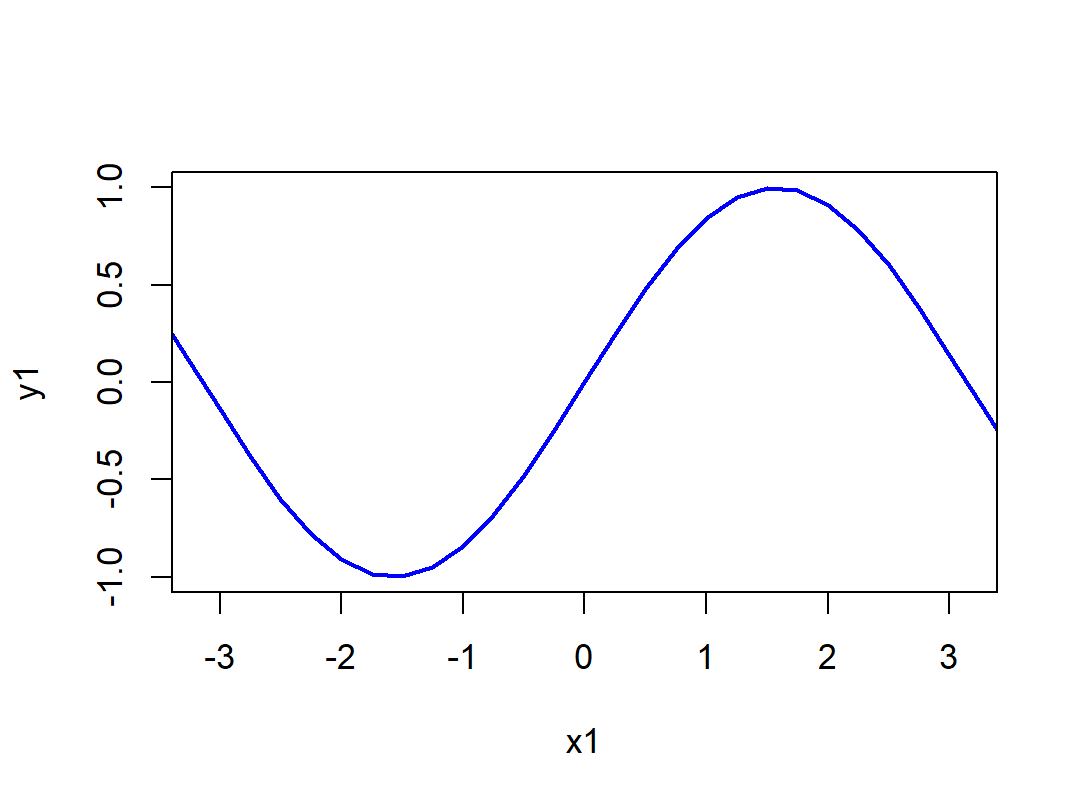
\includegraphics[width=0.65\linewidth,trim={0 0 0 1cm},clip]{images/multiplot_1.png}
\end{center}


\begin{lstlisting}[style=rstyle]
x2 <- seq(-4, 4, by=0.25)
y2 <- x2^2
lines(x2, y2, col = "red", lty = 3, lwd = 4)
\end{lstlisting}

\begin{center}
	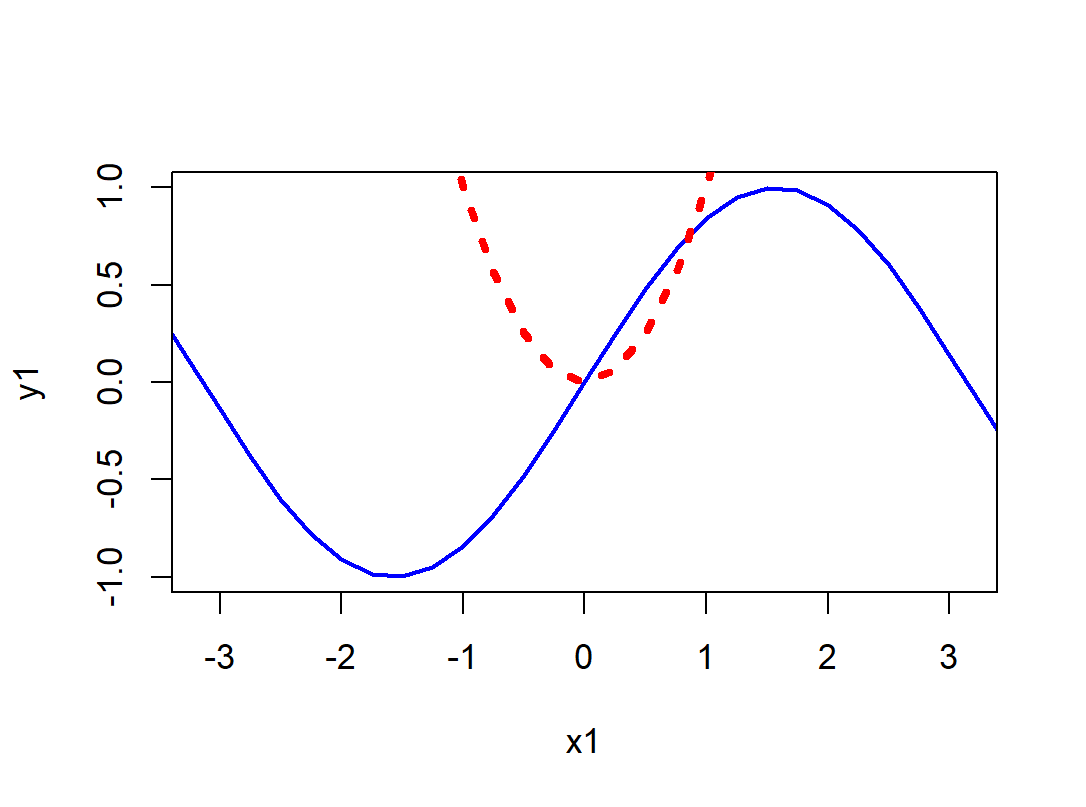
\includegraphics[width=0.65\linewidth,trim={0 0 0 1cm},clip]{images/multiplot_2.png}
\end{center}



\begin{lstlisting}[style=rstyle]
x3 <- c(-3,-3,-2,-2,-1,-1,0,0,1,1,2,2,3,3)
y3 <- c(0.5,-0.5,-1,0,0.5,-0.5,0,1,0.5,-0.5,-1,0,0.5,-0.5)
points(x3, y3, col = "green", pch = 10)
\end{lstlisting}

\begin{center}
	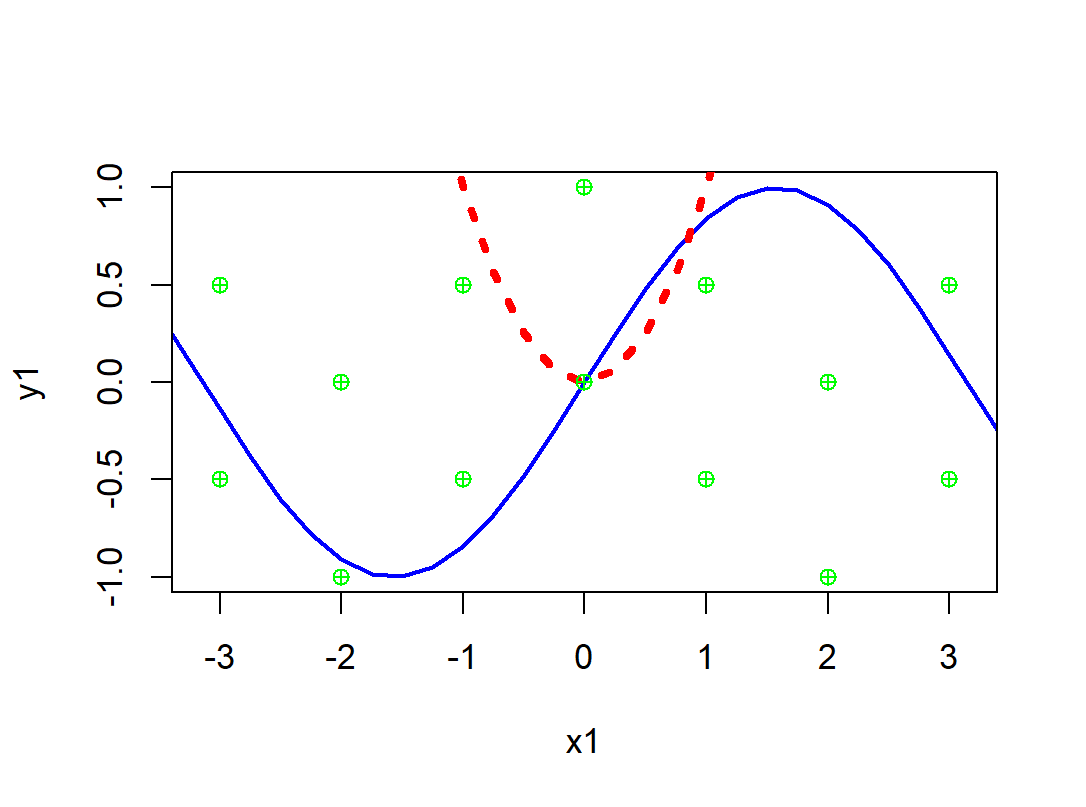
\includegraphics[width=0.65\linewidth,trim={0 0 0 1cm},clip]{images/multiplot_3.png}
\end{center}



\begin{lstlisting}[style=rstyle]
abline(-2,1, col = "orange", lwd = 4)
\end{lstlisting}

\begin{center}
	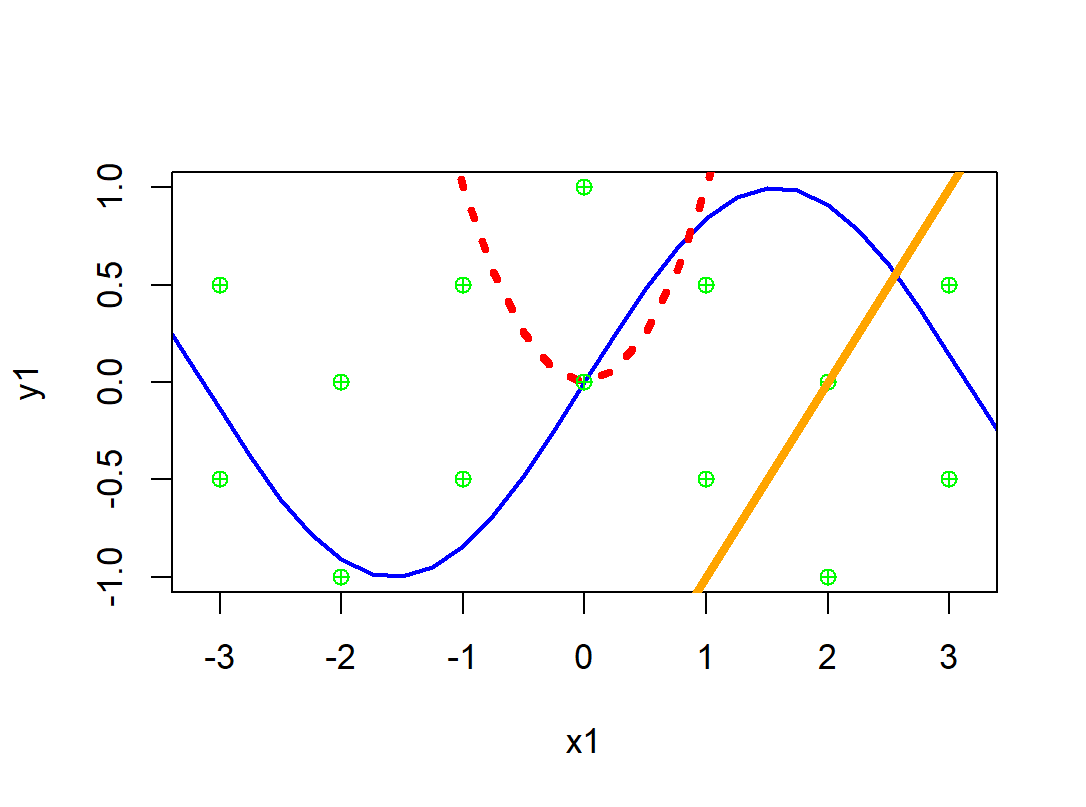
\includegraphics[width=0.65\linewidth,trim={0 0 0 1cm},clip]{images/multiplot_4.png}
\end{center}



\begin{lstlisting}[style=rstyle]
abline(h = 0.5, col = "purple", lty = 2)
\end{lstlisting}

\begin{center}
	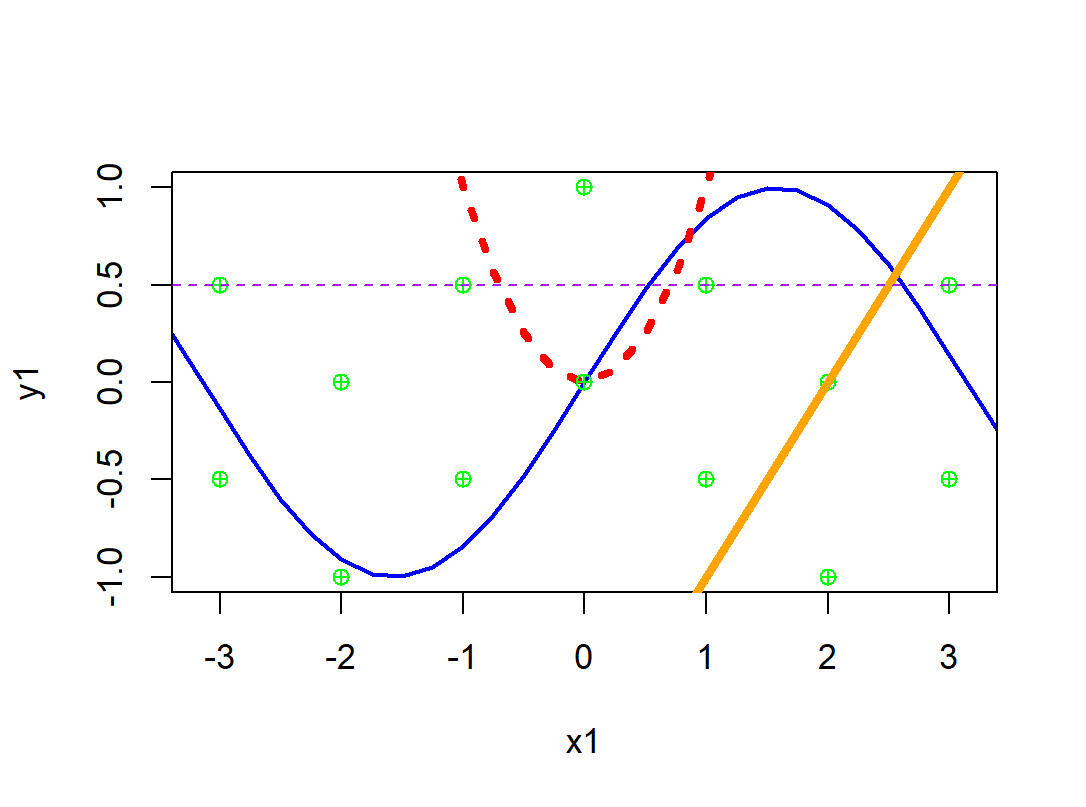
\includegraphics[width=0.65\linewidth,trim={0 0 0 1cm},clip]{images/multiplot_5.png}
\end{center}



\begin{lstlisting}[style=rstyle]
abline(v = -1.5, col = "yellow", lwd = 6, lty = 5)
\end{lstlisting}

\begin{center}
	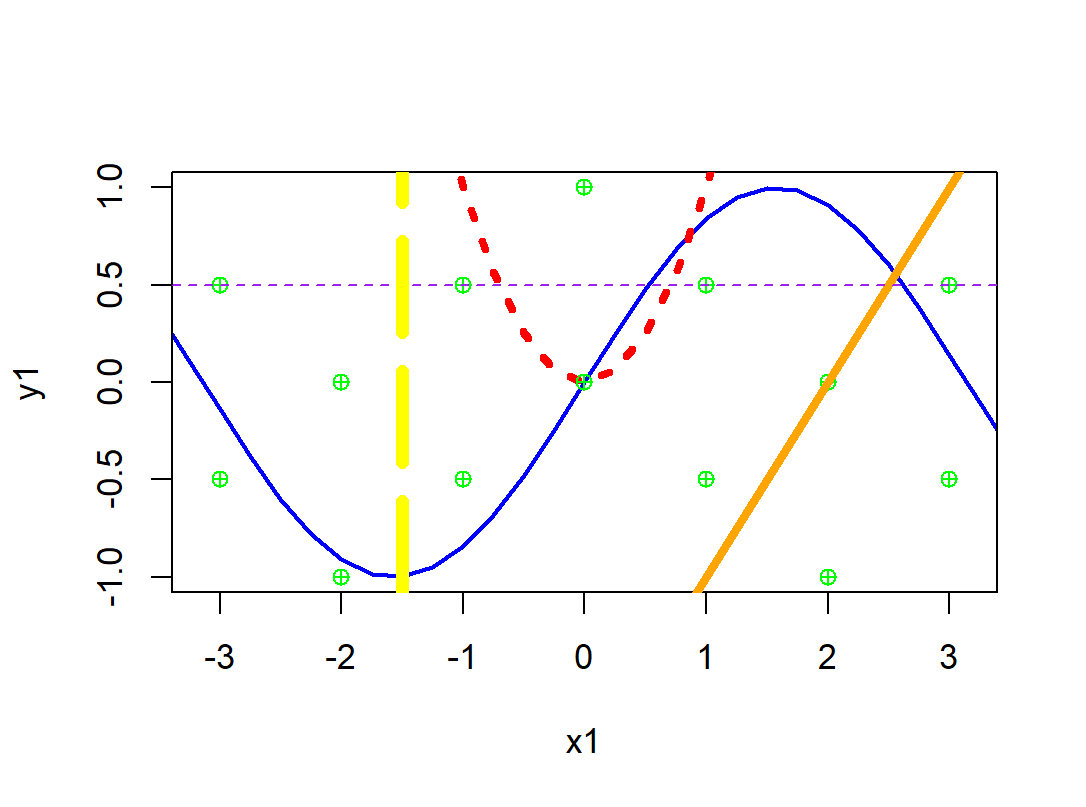
\includegraphics[width=0.65\linewidth,trim={0 0 0 1cm},clip]{images/multiplot_6.png}
\end{center}






\subsection{Leyenda}


Podemos añadir una leyenda con la función \texttt{legend()}. Algunos de sus argumentos son los siguientes:
\begin{enumerate}
	\item Podemos especificar las coordenadas \texttt{x,y} donde queremos que aparezca la leyenda. También podemos usar una posición predefinida como las que se enumeran a continuación:
	\[ \texttt{bottom},\ \texttt{left},\ \texttt{right},\ \texttt{top},\ \texttt{bottomleft},\ \texttt{bottomright},\ \texttt{topleft},\ \texttt{topright}. \]
	
	\item \texttt{legend}: un vector que contiene las etiquetas que describen los elementos del gráfico.
	
	\item \texttt{col}, \texttt{pch}, \texttt{lty}, \texttt{lwd}: vectores que contienen las características del trazo de cada elemento. Cuando no necesitemos especificar nada, usaremos \texttt{NA}.
\end{enumerate}


\begin{lstlisting}[style=rstyle]
legend("bottomright", 
       legend = c("sin(x)", "y = x^2", "puntos arbitrarios", 
                  "recta y = x-2", "recta y = 0.5", "recta x = -1.5"),
       col = c("blue","red","green","orange","purple","yellow"),
       pch = c(NA, NA, 10, NA, NA, NA),
       lty = c(1,3,NA,1,2,5),
       lwd = c(2,4,NA,4,1,6))
\end{lstlisting}

\begin{center}
	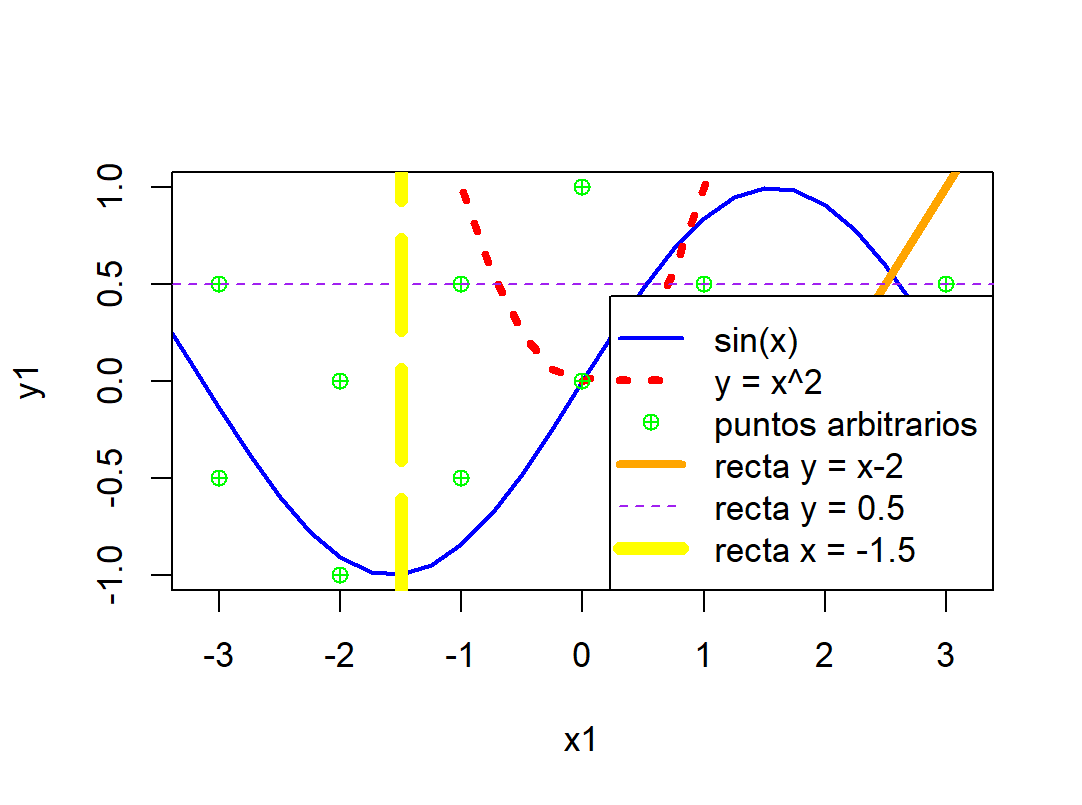
\includegraphics[width=0.65\linewidth,trim={0 0 0 1cm},clip]{images/legend.png}
\end{center}




\subsection{Texto}

La función \texttt{text()} nos permite añadir texto. Sus principales argumentos son:

\begin{enumerate}
	\item Podemos especificar las coordenadas \texttt{x,y} donde queremos que aparezca el texto.
	
	\item \texttt{labels}: contiene el texto a mostrar.
	
	\item \texttt{pos}: posición del texto: \texttt{1}: abajo, \texttt{2}: izquierda, \texttt{3}: arriba, \texttt{4}: derecha.
	
	\item \texttt{cex}, \texttt{col}: tamaño y color del texto.
\end{enumerate}


\begin{lstlisting}[style=rstyle]
text(0,0.5, labels = "Laboratorio", pos = 3,  col = "brown", cex = 1.5)
\end{lstlisting}

\begin{center}
	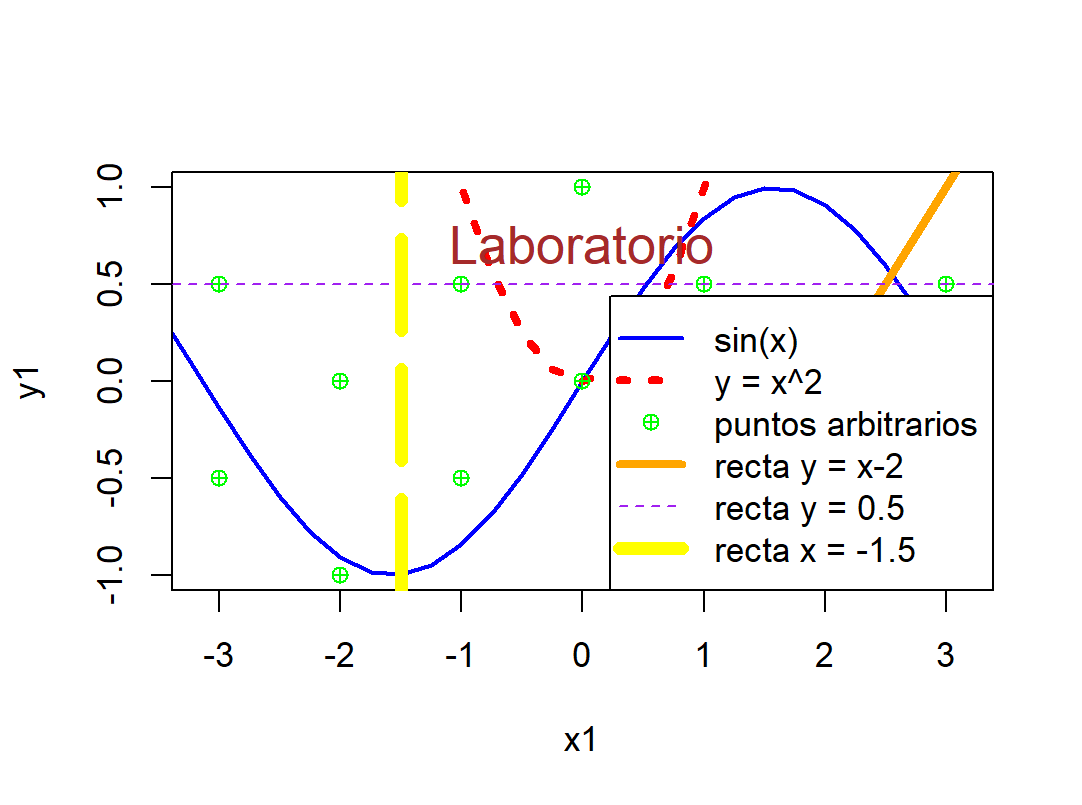
\includegraphics[width=0.65\linewidth,trim={0 0 0 1cm},clip]{images/plot_text_1.png}
\end{center}




\noindent También podemos etiquetar varios puntos al mismo tiempo. Por ejemplo, podemos querer etiquetar los puntos verdes con distintos nombres. En este caso, \texttt{labels} recibiría un vector como argumento.


\begin{lstlisting}[style=rstyle]
text(x3, y3,
   labels = c("A","B","C","D","E","F","G","H","I","J","K","L","M","N"),
   pos = 3, 
   col = "green",
   cex = 1.5)
\end{lstlisting}

\begin{center}
	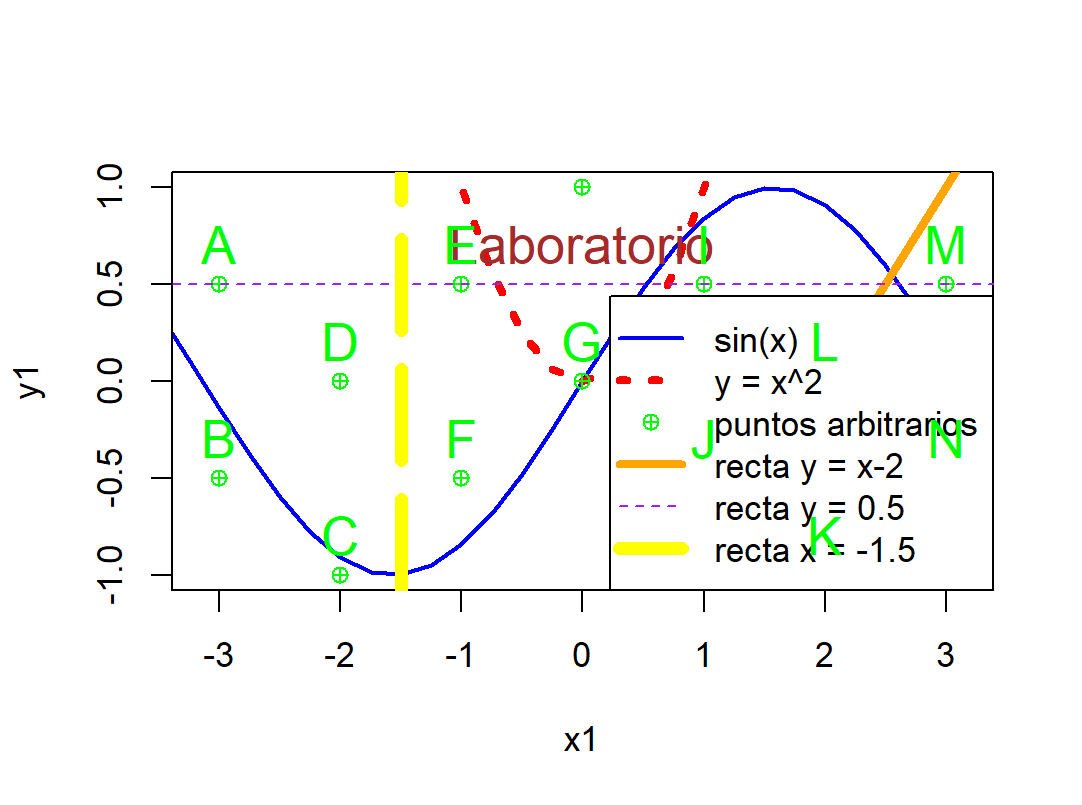
\includegraphics[width=0.65\linewidth,trim={0 0 0 1cm},clip]{images/plot_text_2.png}
\end{center}



\begin{exercise} Representa las gráficas de las siguientes funciones:
\begin{align*}
	y & =1, & y & =\ln(x), & y & =\sqrt{x}, & y & =x, & y & =x \ln(x), \\
    y & =x^3, & y & =x^3, & y & =2^x, & y & = x^x,
\end{align*}
en una única gráfica con \R. El título será \texttt{Complejidades}. Cada función deberá tener un color. Deberás representar únicamente la parte positiva de los ejes $x$ e $y$, esto es, deberás usar \texttt{xlim = c(0,a)} y \texttt{xlim = c(0,b)}, siendo \texttt{a} y \texttt{b} los valores que consideres adecuados. Además, deberás incluir una leyenda que describa todas las gráficas. Las etiquetas que usarás deberán ser de la forma \texttt{O(funcion)}. Por ejemplo, \texttt{O(x·ln(x))} para $y=x \ln(x)$ u \verb|O(2^x)| para $y=2^x$. 
\end{exercise}






\section{Múltiples gráficas}



La función \texttt{par(mfrow)} nos permite construir un gráfico compuesto de varios subgráficos. El argumento \texttt{mfrow} es un vector de dos componentes que especifica la cantidad de filas y de columnas que tendrá la gráfica. Cada vez que se ejecuta una función plot, se rellenará el siguiente subgráfico. Observa el ejemplo siguiente:

\begin{lstlisting}[style=rstyle]
par(mfrow = c(2, 3))

x <- seq(-15, 15, by=0.01)
y1 <- sin(x)
plot(x,y1,type = "l", col = "blue", main = "sin(x)",
     lwd = 2, xlim = c(-2*pi,2*pi), ylim = c(-1,1))

y2 <- cos(x)
plot(x,y2,type = "l", col = "red", main = "cos(x)",
     lwd = 2, xlim = c(-2*pi,2*pi), ylim = c(-1,1))

y3 <- tan(x)
plot(x,y3,type = "l", col = "green", main = "tan(x)",
     lwd = 2, xlim = c(-2*pi,2*pi), ylim = c(-10,10))

y4 <- asin(x)
plot(x,y4,type = "l", col = "orange", main = "arcsin(x)",
     lwd = 2, xlim = c(-1,1), ylim = c(-pi/2,pi/2))

y5 <- acos(x)
plot(x,y5,type = "l", col = "purple", main = "arccos(x)",
     lwd = 2, xlim = c(-1,1), ylim = c(0,pi))

y6 <- atan(x)
plot(x,y6,type = "l", col = "brown", main = "arctan(x)",
     lwd = 2, xlim = c(-10,10), ylim = c(-pi/2,pi/2))
\end{lstlisting}

\begin{center}
	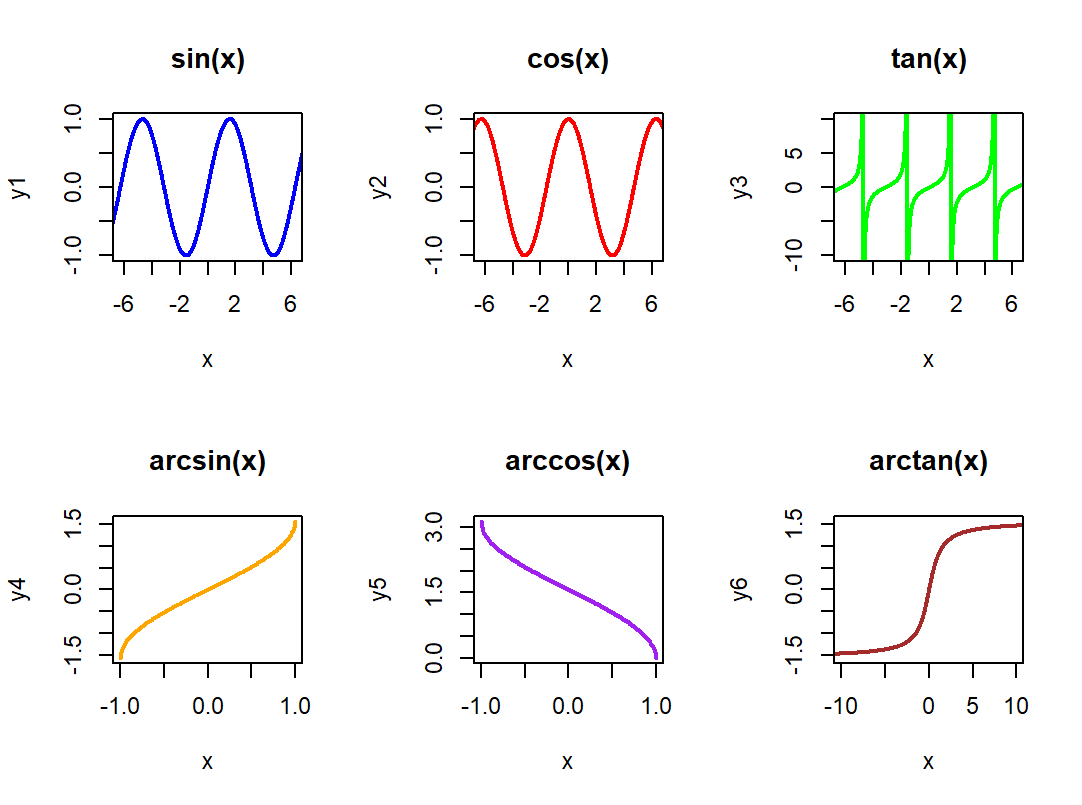
\includegraphics[width=0.9\linewidth]{images/par_mfrow.png}
\end{center}



\begin{exercise} Debes crear las siguientes gráficas múltiples a partir de las gráficas que has generado en el ejercicio 1:
\begin{enumerate}
	\item \textbf{Funciones polinomiales y raíces:} puedes omitir la gráfica del polinomio con exponente $n=6$.
	
	\item \textbf{Funciones exponenciales y logaritmos:} añade la gráfica de la función $f(x) = 2^x$ que has generado en el ejercicio anterior.
	
	\item \textbf{Funciones trigonométricas:} no te limites a copiar el ejemplo. Usa los mismos estilos que has usado en el ejercicio 1.
	
	\item \textbf{Funciones trigonométricas hiperbólicas:} aquellas que acaban en \texttt{h}: \texttt{sinh}, \texttt{cosh}, etc.
	
	\item \textbf{Otras funciones:} el resto de funciones que has representado en el ejercicio 1 y que no están contempladas en el apartado anterior.
\end{enumerate}

\end{exercise}









\section{Documentación del código}
El código debe estar correctamente organizado y comentado. El objetivo no es únicamente conseguir que los gráficos se generen correctamente, sino escribir código fácil de leer y modificar.


\begin{exercise} Crea un fichero \texttt{README.md} para documentar esta práctica. El aspecto deberá ser similar al que encontrarás en la página siguiente.
\end{exercise}


\section*{Entrega}

Sube los ficheros con los ejercicios a tu \GitHub\ en la fecha acordada con el profesor. Para
esta práctica:
\begin{enumerate}
	\item guarda tus scripts en la carpeta de la práctica correspondiente;
	\item utiliza nombres de fichero claros y consistentes;
	\item comenta el código para facilitar su comprensión;
	\item comprueba que puedes ejecutar de nuevo cada script desde el principio;
	\item evita depender de instrucciones que hayan quedado solamente en la consola
\end{enumerate}


\begin{center}
	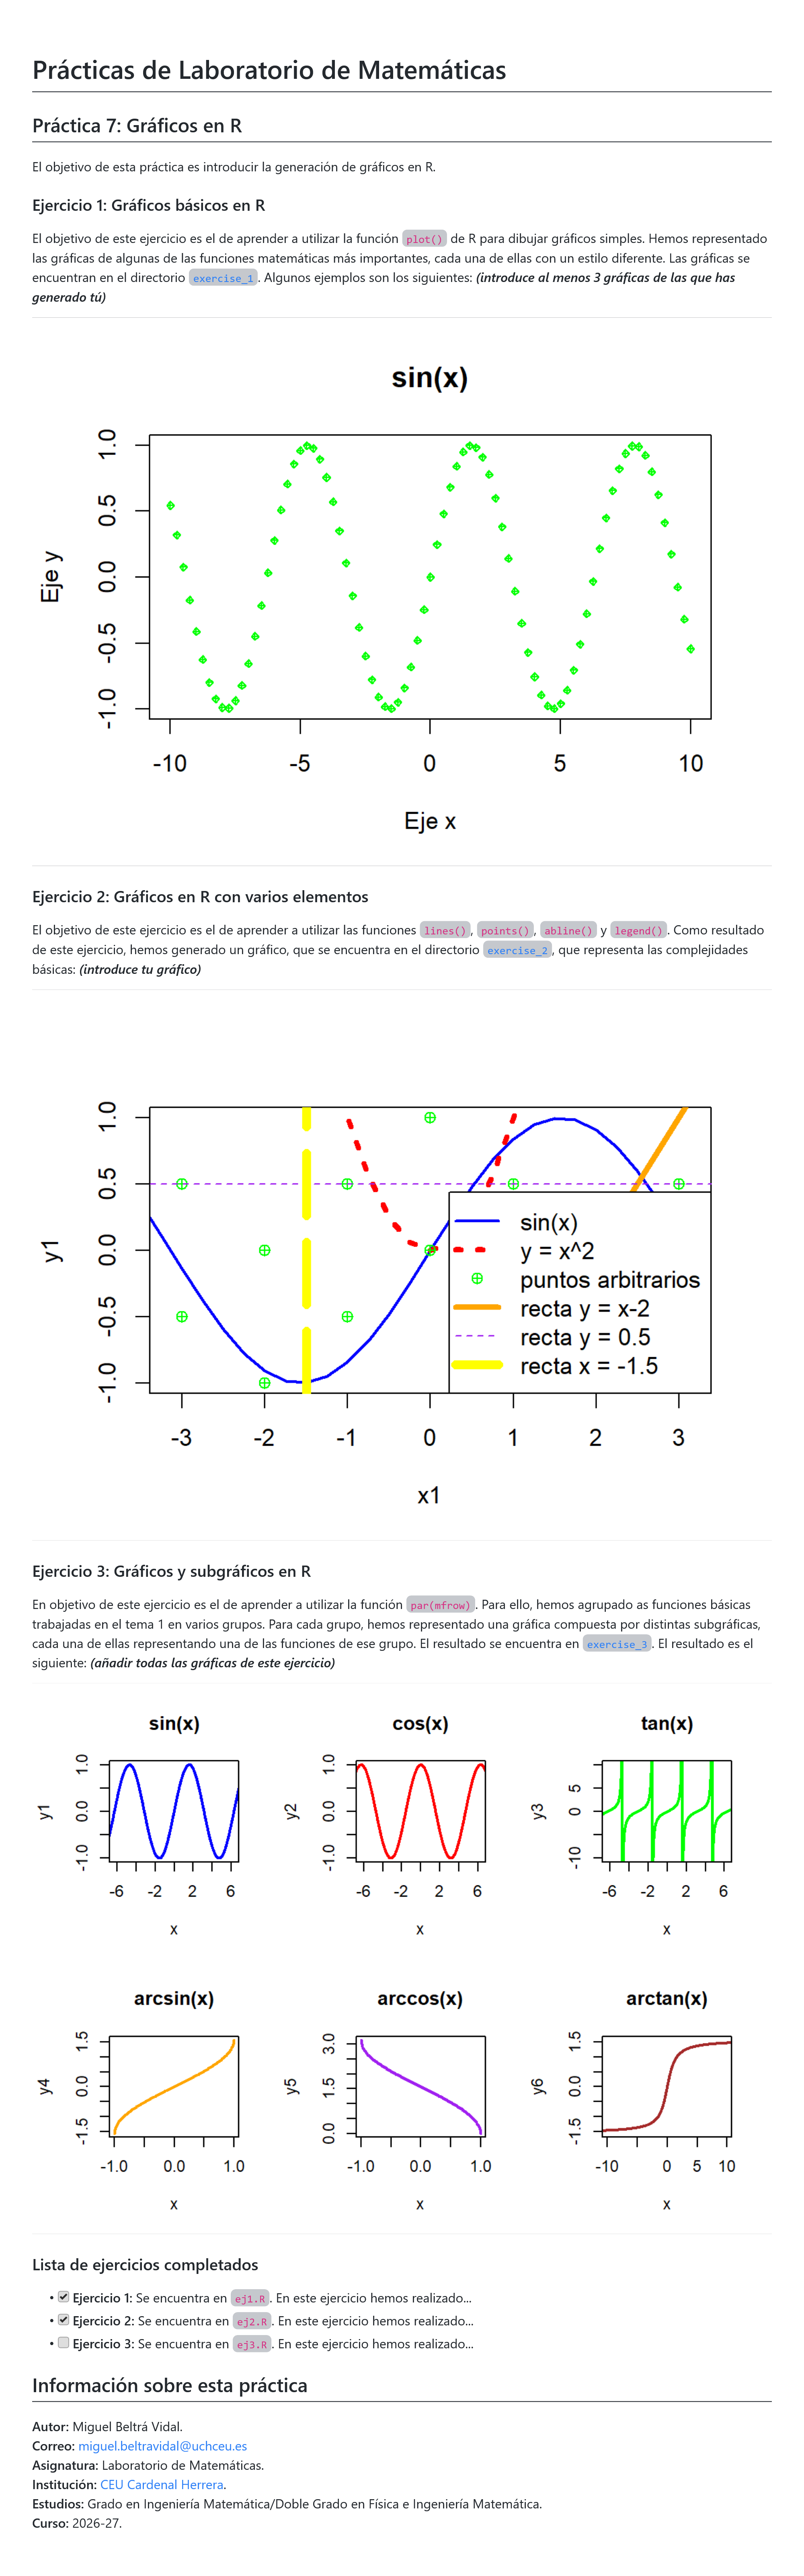
\includegraphics[width=0.5\linewidth]{images/readme}
\end{center}

\end{document}
